\documentclass[swedish,a4paper]{article}
\usepackage[swedish]{babel}
\usepackage[utf8]{inputenc}
\usepackage{amsmath}
\usepackage{amssymb}
\usepackage{algorithm}	   % CODEFormating
\usepackage{algpseudocode} % CODEFormating
\usepackage{csquotes}      % Recommended
\usepackage{graphicx}
\usepackage{wrapfig}
\usepackage{caption}
\graphicspath{ {images/} }
\usepackage[titletoc]{appendix}
\usepackage{listings, listings-rust}
\usepackage{longtable}
\usepackage{tikz}
\usepackage{tikz-cd}
\usepackage[nopostdot,nonumberlist]{glossaries}
\usepackage{pgfplots}
\usepackage{color}
\usepackage[margin=2cm]{geometry}
\usepackage{subcaption}
\usepackage[style=authoryear,
	    sorting=nty,
 	    backend=biber, 
            natbib=true]{biblatex}

\usepackage{hyperref}
\usepackage[swedish]{cleveref}
\usepackage{adjustbox}
\usepackage{float}
% \overfullrule=5pt % for diognosing overflow, draws an black line 

\makeglossaries
\glstoctrue
\newglossaryentry{matris}{
  name=matris,
  description={Data i två dimensioner som en tabell}
}

\newglossaryentry{gsr}{
  name=GSR,
  description={Gilberts-Shanons-Reeds}
}

\newglossaryentry{sd}{
  name=SD,
  description={Standardavvikelse (eng. Standard deviation)}
}

\newglossaryentry{stdmean}{
  name=STDMean,
  description={Standardavviklse-och medelvärde (eng. Standard deviation and Mean)}
}

\newglossaryentry{mp}{
  name=MP,
  description={Medelvärde av Position}
}

\newglossaryentry{pk}{
  name=PK,
  description={Position av Kort}
}

\newglossaryentry{soc}{
  name=SOC,
  description={Shuffle-O-MatiC}
}

\newglossaryentry{df}{
  name=df,
  description={Frihetsgrader (Degrees of freedom)}
}

\newglossaryentry{alfa}{
  name=Signifikansnivå,
  description={Sannolikheten att, vid hypotesprövning, förkasta nollhypotesen trots att den är sann}
}

\newglossaryentry{pvalue}{
  name=\(p\)-värde,
  description={Den uppmäta sannolikheten att nollhypotesen är sann}
}

\newglossaryentry{ns}{
  name=ns,
  description={Nanosekunder}
}

\newglossaryentry{apen}{
  name=ApEn,
  description={Approximate entropy}
}

\newglossaryentry{bibliotek}{
  name=bibliotek,
  description={Samling av färdigt byggt kod för programmerings språk Python}
}

\newglossaryentry{crate}{
  name=crate,
  description={Samling av färdigt byggt kod för programmerings språk Rust}
}

\newglossaryentry{prng}{
  name=PRNG,
  description={Pseudoslumptalsgenerator}
}

\newglossaryentry{trng}{
  name=TRNG,
  description={Äkta slumptalsgenerator}
}


\pgfplotsset{compat=1.14}
\lstset{ % General settings for listings
	basicstyle=\ttfamily\small, 
	commentstyle=\color{green},
	keywordstyle=\color{blue},
	stringstyle=\color{red},
	tabsize=4,
	% numbers=left,
	% stepnumber=1,
	% numbersep=-10pt,
	% numberstyle=\small\color{gray},
	showstringspaces=false,
	breaklines=true,
	showspaces=false,
}

% Redefine the listing name after loading cleveref
\renewcommand{\lstlistingname}{Kodlistning}
\crefname{lstinputlisting}{kodlistning}{kodlistningar} % For cleveref, singular and plural
\Crefname{lstinputlisting}{Kodlistning}{Kodlistningar} % For cleveref, singular and plural, capitalized

\renewcommand{\algorithmicrequire}{\textbf{Indata:}}
\renewcommand{\algorithmicensure}{\textbf{Utdata:}}
\renewcommand{\listalgorithmname}{Algoritmlista} % Ändrar "List of Algorithms" titel
\floatname{algorithm}{Algoritm} % Ändrar "Algorithm" till "Algoritm" i rubrike

\addbibresource{references.bib}
\renewcommand{\appendixpagename}{Bilagor}
\renewcommand*{\bibfont}{\small} % Adjust font size
\setlength{\bibitemsep}{1.5em} % Increase space between entries
\setlength{\bibhang}{2em} % Indent bibliography entries

\renewcommand*\contentsname{Innehåll}

\newcommand{\boldsection}[1]{%
  % \vspace{5mm}% Add some vertical space above the section
  \small\textbf{#1}% Make the text bold
}
 % Custom commands

\begin{document}

\begin{titlepage}
	\begin{minipage}[t]{0.45\textwidth}
		\raggedright
		NTI Gymnasiet - Nacka Strand \\
		Teknikprogrammet-Teknikvetenskap \\
		Gymnasiearbete 100p \\
		HT 2023 - VT 2024
	\end{minipage}
	% \hfill
	\begin{minipage}[t]{0.5\textwidth}
		\raggedleft
		\begin{adjustbox}{valign=t}
			
\includegraphics[width=\linewidth]{logo.png}
		\end{adjustbox}
	\end{minipage}

	\vspace*{\fill} % Add vertical space to center the title

	\begin{center}
		\Large\textbf{En ny potentiell automatiskt kortleksblandare}\\
		\large\textit{Proof of Concept av en kortblandare}
	\end{center}

	\vspace*{\fill} % Add vertical space to center the title

	\begin{minipage}[b]{0.45\textwidth}
		\raggedright
		Namn: Eduards Abisevs\\
		E-post: eduards.abisevs@elev.ga.ntig.se\\
		Namn: Leo Altebro\\
		E-post: leo.altebro@elev.ga.ntig.se\\
		Handledare: Elias
	\end{minipage}
	\begin{minipage}[b]{0.5\textwidth}
		\raggedleft
		Typsatt med \LaTeX. \\
		Kompilerad \today.
	\end{minipage}
\end{titlepage}

\begin{center}
    \large
    \vspace{0.9cm}
    \textbf{Abstract}
    \vspace{0.9cm}
\end{center}
Lorem ipsum dolor sit amet, consectetur adipisicing elit, sed do eiusmod tempor
incididunt ut labore et dolore magna aliqua. Ut enim ad minim veniam, quis
nostrud exercitation ullamco laboris nisi ut aliquip ex ea commodo consequat.
Duis aute irure dolor in reprehenderit in voluptate velit esse cillum dolore eu
fugiat nulla pariatur. Excepteur sint occaecat cupidatat non proident, sunt in
culpa qui officia deserunt mollit anim id est laborum.

\tableofcontents
\newpage

\glsaddall[] % adds all ordlist.tex entries
\printglossaries % Ordlista printas här
\newpage

\section{Inledning}
\subsection{Introduktion till ämnet}
Spelbranschen är en industri som omsätter miljardbelopp och precis som alla
industrier utvecklas den med resten av världen. Industrier över hela världen har
som mål att hitta nya sätt att effektivisera och sänka kostnad på det arbete som
utförs för att bedriva vinst, och spelbranschen har följt denna långvariga trend
med till exempel online casinon. Inom spelbranschen är kortspel vanligt
förekommande, att försöka automatisera dem är därför ett logiskt steg att ta, men för
en stor industri vill man vara extra säker på att allt utförs på bästa sätt.
Alla sätt att blanda kort är nämligen inte lika bra, vilken sorteringsmetod som
används kan ha påverkan på resultatet. Teknologins inflytande inom spelbranschen
ökar kraftigt, de största delarna av branschen bedrivs mer och mer av maskiner
och algoritmer som får stor potentiellt inflytande på spelresultat, därför är
det bäst att börja tänka på möjliga problem så snart som möjligt. Redan nu finns
det blandningsmaskiner för kortlekar som vi inte vet någonting om; varken hur de
funkar eller hur bra de är. Allt som vi vet är de är certifierade av
tredjepartsföretag. Faktumet att de kan kosta upp till 100 000 kr betyder att
inte vem som helst kan ha tillgång till en kortblandningsmaskin.

\subsection{Syfte}
\label{sec:purpose}
Syftet med denna undersökning är att ta fram den hypotetiskt bästa kortblandaren
utifrån två faktorer: 1) hur slumpmässigt den algoritm som den byggs efter kan
blanda kort; 2) till vilken grad den potentiella maskinen byggd efter algoritmen
skulle fungera i verkligheten. Med resultaten förväntas variationen i
slumpmässighet för olika blandningsmetoder kunna visas upp samt kunna använda de
resultaten för att komma fram till den hypotetiskt definitiva maskinen, något
som är viktigt då spelbranschen handlar mycket om chans. Det är därför viktigt
att se till att allt funkar på bästa sätt. I den här vetenskapliga rapporten
kommer en jämförelse av hur effektivt framtagna blandningsmetoder kan fungera i
en hypotetisk blandningsmaskin att utföras. Samtidigt som man kan utforska hur
en dator kan göra slumpmässiga sekvenser på ett effektivt sätt med tanken att
den ska tillämpas till en potentiell kortblandare. Detta är viktigt för att
spelbranschen är en stor industri som handlar mycket om tur, att se till att de
slumpmässiga resultaten är framtagna på bästa möjliga sätt är en essentiell del.
Vi söker med hjälp av data svaret på frågan:

Utifrån slumpmässighet och effektivitet, vilken kortblandningsmetod är bäst för
en potentiell spelkortsblandare som uppfyller följande:
\begin{itemize}
	\item Fysiskt tillämpning: Hur pass väl den kan framställas i verkligheten 
	\item Effektivitet: Utifrån mjukvaras och hårdvaras perspektiv
        \item Kortblandnings slumpmässighet
\end{itemize}


\section{Teori}
\subsection{Beräkningsteori}

Beräkningsteori är en del av matematik vars syfte är grundat i hur och om
problem kan bli lösta på olika beräkningssätt. Beräkningsteori har flera olika
grenar. En gren handlar om vad som går att bevisa inom matematik angående om
nummer och funktioner är beräkneliga eller inte. Med beräknelig menas något som
kan beräknas, det vill säga värderas, uppfattas eller förutses, när det kommer
till matematik syftar det på att bestämma något via matematiska
modeller eller processer, alltså att kalkylera.

\subsection{Slumpmässighet}
\label{sec:slump}

Slumpmässighet är en egenskap som anger att något sker utan klart mönster. När
något är helt slumpmässigt är det i princip omöjligt att förutse. Slumpmässighet
inom matematik är byggd beräknings\-teori och den delas upp i två beroende på om
det gäller slumpmässighet av en bestämd mängd eller en oändlig mängd av objekt
\parencite[49-66]{Terwijn2016}.

\subsection{Bakgrund av blandings metoder}
Theoretical Whats, Whys and Hows angående algorithmer.

\subsubsection{Riffle shuffle}
\label{sec:riffle_shuffle}
% Riffle Shuffle är den mest kända kortleksblandningsmetoden.
Det finns många olika metoder att blanda kort med riffle shuffle.
Gilbert-Shannon-Reeds-modellen är en matematisk modell på riffle shuffle som ger
resultat nära dem en riffle shuffle utförd av en människa ger.

\begin{figure}[H]
	\begin{center}
		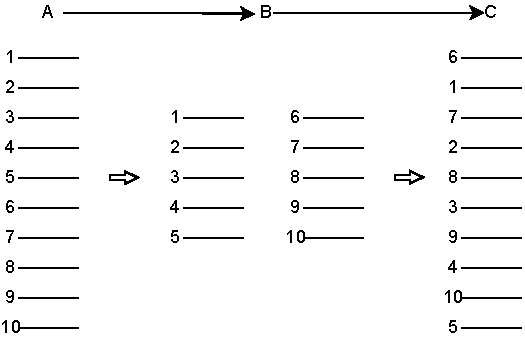
\includegraphics{images/rifflle-shuffle.pdf}
	\end{center}
	\captionsetup{justification=centering,margin=2cm}
	\caption{Steg i processen för Riffle Shuffle. Illustrationen visar de
	iterativa stegen från den ursprungliga högen (A), uppdelning i två
	högar (B), infoga dem två högarna med varandra för att bilda en ny hög.
        Pilar indikerar riktningen för blandningsprocessen.}
	\label{fig:riffle_shuffle_1}
\end{figure}

% \begin{algorithm}
% \caption{Riffle Shuffle Pseudokod}
% \begin{algorithmic}[1]
% \Require $Deck$
% \Ensure Blandad $Deck$
% \For {$card$ in len($Deck$)} { 
% \State $DeckHalf1.push(card) $ 
% \State $DeckHalf2 \gets $
% }
% \State Initialize an empty list $ShuffledDeck$
% \While{both $DeckHalf1$ and $DeckHalf2$ are not empty}
%     \State Generate a random number $RandId$ between 0 and 1
%     \If{$RandId \leq$ length of $DeckHalf1$ divided by total length of both halves}
%         \State Remove the top card from $DeckHalf1$ and add it to $ShuffledDeck$
%     \Else
%         \State Remove the top card from $DeckHalf2$ and add it to $ShuffledDeck$
%     \EndIf
% \EndWhile
% \State Copy $ShuffledDeck$ back to $Deck$
% \end{algorithmic}
% \end{algorithm}

\subsubsection{Pile shuffle}
\label{sec:pile_shuffle}
Pile shuffle är en kortleksblandingsmetod som genomförs med fysiska
kort. Processen utgår från att ett kort
från kortleken läggs i en av flera olika högar. Processen försätter
tills alla kort från kortleken har flyttats till en av högarna. Sedan
läggs  alla högar ihop i en ny kortlek. 


\begin{figure}[H]
	\begin{center}
		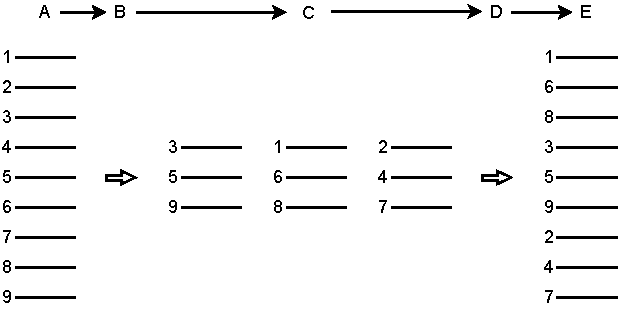
\includegraphics{images/pile_shuffle.pdf}
	\end{center}
	\captionsetup{justification=centering,margin=4cm}
	\caption{Steg i processen för Pile Shuffle. Illustrationen visar de
	iterativa stegen från den ursprungliga högen (A), genom uppdelning i
	högar (B), temporara högar (C), omarrangering av temporara högar (D),
	och tillbaka till en enda hög (E). Pilar indikerar riktningen för
	blandningsprocessen.
	}
	\label{fig:pile_shuffle_1}
\end{figure}


\subsubsection{Inblick i en professionell kortlkesblandare}
\label{sec:wheel}


\subsection{Klassiskt poker test}
\label{sec:poker_test}


% Poker Test kan anpassas till vilken som helst sekvens av nummer 3-5 stora
% mängder. Men för att vår simulation använder vi samma nummer som pokerkort
% därför kan vi anpassa klassiska poker test var man använder alla möjliga
% pokerhänder av sekvens av 5 kort. Resultatet från karakterisering av händer
% använder man i en chi-square testet. För att göra testet rätt följde jag
% Engineering Statistics handbok (NIST 2012). Dvs för att avgöra hur många 
% händer
% uppkom med avseende till teoretiska värdena EXPECTED vs OBSERVED värdena. sen
% jämför man chi-square resultatet till en CRITICAL värde om den värden som vi
% fick är mindre kan vi med säkerhet säga att algoritmen är slumpmässigt och 
% vice versa.

Ett klassiskt poker test används att avgöra slump\-mässighet i numeriska 
sekvenser, oftast för att testa slumptalsgeneratorer. Testet utförs genom
att 3 till 5 nummer väljs ut ur en sekvens och placeras i en av sju
kategorier beroende på mönstret som talen har.  Mönstren är baserade på händer i poker vilket är varför testet kallas poker test \parencite{Abdel2014}. 
De olika mönster som letas efter i talen visas i Tabell \ref{tab:num_poker_hands}.
\begin{table}[H] 
	\centering
        \caption{Vanliga kategorier till poker test}
        \label{tab:num_poker_hands}
	\begin{tabular}{|l|c|}
	\hline 
	Pokerhand & Mönster \\ \hline  
	Femtal & AAAAA \\ \hline
	Fyrtal & AAAAB \\ \hline
	Kåk & AAABB \\ \hline
	Tretal & AAABC \\ \hline
	Tvåpar & AABBC \\ \hline
	Par & AABCD \\ \hline
    	Ingen mönster & ABCDE \\ \hline
	
\end{tabular}

\end{table}
\noindent
 Antalet mönster i varje kategori räknas för att få en distribution, som
 då jämförs med en distribution som stämmer överens med sannolikheten
 att få de olika mönstren. Om det total antalet mönster är $n$ och
 sanolikheten för en pokerhand $i$ är $p_i$, därför borde antalet mönster i
 den kategori vara $$e_i = p_i * n$$ Där $o_i$ är antalet mönster som
 borde matcha pokerhand $i$. För att bestäma om resultaten kan komma
 från en rättvis kortlek jämnförs de resultat som fåtts av att plocka
 ut nummer mot de resultat som fås av sannolikheten via ett chi-två-test.

\begin{equation*}
\end{equation*}

\subsubsection{Chi-två-test}
\label{sec:chi_square}
Inom statistik används ett \textit{goodness-of-fit} test för att mäta
hur pass väl fördelningen för den data som observerats stämmer överens
med fördelningen som data förväntas ha utifrån en model. Karl Pearsons
chi-två-test kan användas som \textit{goodness-of-fit} test. Det
använder chitvåfördeling. I testet jämnförs ett värde $\chi^2$ med ett
kritiskt värde för att bestäma om den observerade följer den förväntade
fördelningen. $\chi^2$ beräknas enligt formeln
$$\chi^2 = \sum_{i=1}^k\frac{(O_i - E_i)^2}{E_i}$$
Där $O_i$ är observerade frekvensen för en kategori av data $i$ och $E_i$
är förväntade frekvensen för kategorin $i$ \parencite{nist}.
Det kritiska värdet fås av antalet frihetsgrader(kategorier - parametrar)
och signifikansnivån som bestämts för testet.

Ett aspekt i chi-två-test är att data mängderna som testas inte kan vara för
små. Det rekommenderas att $O_i$ inte är mindre en 5.

%Chi-square, chi-två testing eller som den också betecknas $\chi^2$ är statistikt test
%som oftas används till att definera och beräkna slumpmässighet av bestämd sannolikhet.
%$$ \chi^2 = \sum_{i=1}^k \frac{(O_i - E_i)^2}{E_i}$$
%Vart $O_i$ är observerade frekvensen för kategorin $i$ och $E_i$ är förväntade
%frekvensen för kategorin $i$ \parencite{nist}.
\subsection{Standardavvikelse- och medelvärdestest (STDMean) testet}
\label{sec:stdmean}
Datamängden är utformat på sätt att kort värde är alltså dess position i
kortleken. Första kort är 0 dvs position 0 i kortleken. Kalkylerar varje
columns korts medelvärde och standaravvikelse ska man förustpå att medelvärde
borde ligga nära $51/2= 25.5$ detta betyder att i position 0 har alla kort varit
i, och om standaravviklse i figuren är höga torn har position 0 stort variation
av vilka kort som var där. Detta är då en indikator på en uniform distribution
som betyder en slumpmässigt algoritm.

Förklara logiken till stanardavvikelse och medelvärdet
i logiken med avgörande av normal distribitution och hur den ger ett mått/bild på randomness

\subsection{Pseudoslumptalsgenerator (PRNG)}
\label{sec:prng}
Här berätta om ChaCha20 \parencite{chacha} den som är biobliotekes rand
\parencite{rand_crate} default PRNG och mersenne twister som egentligen var första
hands val
\parencite{mersenne_twister} men som vi sedan bytte till ChaCha för att i rust
är det relativt svårt att  implementera och använda mersenne twister. Berätta om
dem skillnaderna som finns.


En väldigt känd och testad algoritm är Mersenne Twister (MT 19937) som
har en väldigt långt period innan siffrorna börjar att upprepa sig, mer
exakt $2^{19937}$ \parencite{mersenne_twister}.

Alltså nämn att för att det här är som et proof of concept, borde vid
senare tillfälle användas en hårdvara PRNG och icke software PRNG.
Men på grund av detta undersökning handlar mesta dels om stora mängder av data
simulationer så måste vi använda och "Sacrifice" verkliga till att lättare
skapa simulationer!

\subsection{Programmerings verktyg}
\label{sec:verktyg}
Python är en objektorienterad, dynamiskt typad programmerings språk med
fokus på läsbarhet med en enkelt syntax \parencite{python}. Detta  som tillför att det finns stora
mängder av biblioteker (samling av färdig kod).
Python används ofta i statiskt och numeriskt analys på grund av dens
läsbarhet och lätt använding. På grund av Python är skriven i
programmeringspråket C finns det också tilgännliga C API's med andra
betecknat CPython. Dem gör det möjligt att skapa program som är snabba
och effektiva i stora datamängd analys. Dessa egenskaper har medföljt
början av skapande av tiotals avancerade numeriska och
bibliotek som är snabba i utförande och minskar antal radar av kod som
behövs att skrivas i färdigt program. Dem bibliotek som är speciellt
intressenta i detta undersökning är NumPy, Matplotlib, SciPy och Numba.
NumPy som är snabbt i vektoriserad aritmetik och SciPy som har många
inbygga statistiska tester som $\chi^2$-testet \parencite{numpy, scipy}.


% grund av dens rika utbud av bibliotek, speciellt inom
% veten\-skaplig data\-behandling och data\-analys. Därför valdes det
% att utföra statistika tester som Poker test och \gls{stdmean} testet i Python.
% En till perspektiv till varför Python valdes är att analys och avgörande
% av slump\-mässighet är fundementalt komplex process icke räknebart, men det som
% underlättar framtagande av resulat är visuella grafer och tabeller. I

% Med detta sagt Pythons Matplotlib bibliotek underlättar processen av
% graf ritanade tillsammans i en symbious relation med NumPy som har styrka i
% datamängd represention och vektoriserad data\-bearbetning. Utfördes det
% mindre matematisk komplicerade tester med fokus på storleken av
% datamägderna som ger en god överblick av slumpmässighet av dem olika
% blandnings algoritmerna som simulerades. På avseende på ett teoretiskt
% perfekt blandnings resulat för samtliga metoder.

Rust är ett programmeringsspråk som fokuserar på
minnessäkerhet, parallellism och minneseffektivitet. Rust är känt för
sina avancerade funktioner som ägarskapssystemet (ownership), vilket
hjälper till att förhindra minnesläckor och tillåter säker
minneshantering utan en skräpsamlare (garbage collector)
\parencite{rust}. Detta har ökad populäritet i användning av Rust i
inbyggda system som ett motkandidat till c/c++. 

\section{Metod} 
Metoden för denna studie kan indelas i tre huvudområden
1) Framtagande av  blandningsalgoritmerna. 
2) Simulering av kortblandningsprocesser. 
3) Statistisk analys av insamlad data.
% Målet är att besvara en av frågestälningens kriterium "Kortblandnings
% slumpmässighet ".

Inledningsvis kommer framtagande av blandningsalgoritmerna fokusera på
utvecklingen av specifika kortblandningsmetoder. Detta inkluderar både
etablerade metoder som Riffle Shuffle (\ref{sec:riffle_shuffle}), samt nyare,
innovativa tillvägagångssätt som Pile Shuffle (\ref{sec:pile_shuffle}). Såsom
anpassning av design av en professionell kortleksblandare (\ref{sec:wheel}).
Vilka valts ut baserat på deras potential i en potentiell kortleksblandare.
Dessa algoritmer är kritiska för bedömningen av kortblandningsmotodens
slumpmässighet och effektivitet, vilket är kärnan i studiens frågeställning. 
% Samt att besvara
% frågan om dess algoritmernas fysiskt tillämpning i en potentiell
% kortleksblandare.

Målsättningen med denna sektion är att djupgånade undersöka kortblandnings
fysiskt tillämplighet, dess effektivitet och slumpmässighet. Att utföra 
simulation valdes därmed att blandningsalgoritmerna
(processmässigt) skulle vara snarlika till dess potentiella kortleks\-blandare.
Därmed skulle det genereras mer tillförlitliga testresultat. Därför simuleringsdelen
innefattar en kvantitativ metodik för att reducera den inneboendes
slumpvariation i de simulerade blandningsalgoritmerna. Genoma att generera ett bestämt
mängd av kortleksblandningar, där datamängder uppfyler kravet ifrån statistiska metoder. Dessa
statistiska  analysmetoder omfattar det klassiska pokertestet (\ref{sec:poker_test}), med
resulat given av chi-två-testet (\ref{sec:chi_square}). Samt \gls{stdmean} testet
(\ref{sec:stdmean}), vilket ger ett närmare inblick i korts variation i specifika
positioner i kortleken. Tillsammans dessa tester ger en tillfredsställande indikation på
blandningsmetodens slumpmässighet. 

Genom att välja denna metodik syftar studien till att utföra en omfattande
kvantitativ analys som inte enbart bedömer algoritmernas teoretiska
effektiviteten men även dess praktiska tillämplighet i en potentiell kortleks\-blandare.
Detta tillvägagångssättet möjliggör en detaljerad utvärdering av varje algoritm,
dess implementering och slutliga prestande, vilket är avgörande för att uppnå
studiens mål. Mer detaljerad beskrivning av specifika algoritmerna,
simuleringar av kortblandningar och statistiska utvärderingar presenteras i kommande 
underrubriker. 

För intresserade parter finns det källkod för algoritmernas implemention,
programmet som användes för simulation, samt implementionen av analysmetoderna
på Github se Bilaga \ref{app:github}.

% Valet av metodik syftar till att implementera blandsnigsalgoritmerna med syfte
% att motivera design valet och framställa dem med tanken att dessa skulle
% implementeras i ett potentiell kortleksblandare. Sedan  genomföra en 
% kvantitativ analys med användning av 
% simuleringar och statiska utvärderingar. Simulationen  Datamängden kakylerades med avseende på krav i det klassika
% pokertestet. Dessa metoder är detaljerat beskrivna i respektive underrubrik.
% under sin livscykel.
%
% Simulationen omfatar ett  för att minimera
% naturligt slumpmässighet i statiska metoder som ska tillämpas. Dessa 
% metoder är Klassikt poker test
% med resultat given av chi-två-fördelning respektive \gls{stdmean} testet.
% ett närmare undersökningen av 
% korts variationen  i alla positioner i kortleken med statiska metoder som standardavvikelsen,
% respektive medelvärdena av korts position.
%
% Detta metod valdes för att utföra ett kvantitiv undersökning med
% hjälp av simulation och statistiska tester.  
% dvs på liknande sätt hur ett fysiskt kortleks\-blandare skulle används under dens livscykel. 


\subsection{Testmiljö} 
I valet av testmiljö prioriterades operativsystemets kompatabilitet av
de utvecklingsverktyg som användes. Linux valdes på grund av dess
robusta stöd för programmeringsmiljöer och breda stöd för
mjukvaruutvecklingsverktyg. Dessutom erbjuder operativsystem Linux bättre kontroll
över systems\-resurer, vilket är avgörande för att uppnå följdriktiga
och till\-för\-litliga testresulat. Därför utfördes undersökningen på en
 dator med  Linux som operativsystem. Se se Tabell \ref{tab:linux_env} för
 testmiljös specifikationerna.
\begin{table}[H]
\centering
\begin{tabular}{|l|p{5cm}|}  
\hline 
Typ & Specifikation  \\ \hline 
Processor & AMD Ryzen 5 3600 \newline 6 cores / 12 threads \newline 3.6 GHz \\ \hline
RAM & 15.93 GB \\ \hline
Hårddisk & KINGSTON SA400S3, 447 GB \\ \hline
Operativsystem & \texttt{Arch Linux x86\_64, \newline Linux kernel
6.6.9-arch1-1} \\ \hline
\end{tabular}
\captionsetup{width=0.5\textwidth}
\caption{Testmiljö med Linux som operativsystem.}
\label{tab:linux_env}
\end{table}

\subsection{Framtagande av blandningsalgoritmerna}
\label{sec:algos}
I detta avsnitt presenteras processen av framtagande och 
% kortblandningsalgoritmerna som utgör studies kärna. Här teoretiska grunden för
% Riffle Shuffe (\ref{sec:riffle_shuffle}), Pile Shuffle (\ref{sec:pile_shuffle})
% och design ifrån profesionell korleksblandare (\ref{sec:wheel}) kommer att
% anpassas till en potentiell kortleksblandare och implementeras för vidare undersökning. 
detaljerna kring varje algoritms kod och dess
möjliga implementering i en potentiell kortleksblandare.
% kommer att utforskas.
% vilket lägger grunden för en djupare analys av deras prestanda i efterföljande
% simulationer och analysmetoder.

Algoritmerna implementerades i programmerings språk Rust version 1.73.0. Rust
valdes p.g.a dess höga abstraktioner med närmare tillgång till systemresurer
(för detaljer se avsnitt \ref{sec:verktyg}). Därmed att i ett fysiskt maskin
skulle blandningsalgoritmeren köras i ett inbyggd miljö det vill säga i system med
begränsade resurser. Dessutom på så sätt implicit skapas det en mer likvärdig till en
potentiell kortblandingsmaskin miljö för efterföljande simulationer. 

Kompromisen som togs i implementation av algoritmerna är att
pseudoslumptalsgenerator (\gls{prng}) som används i denna studie kommer ifrån
Rand \gls{crate} som har inbyggt implemention av ChaCha20 (se sektion
\ref{sec:prng} för detaljer). Som tidigare nämnts behöver ChaCha20 mer
systemresurer och därför är inte tillgängligt i ett inbyggt system. Men
valet av att använda denna togs för att i simulerings miljö där \gls{prng} behövs
successivt i små tids intervaller kommer den att generera bättre pseudoslumptal
än en \gls{prng} som är anpassad till inbyggda system. Dessutom kommer den att
generera mer trövärdiga kortblandingar som är mindre influenserade av dess
underliggande \gls{prng} implemenation. 

\subsubsection{Anpassning av Riffle Shuffle}

 
\begin{wrapfigure}{r}{0.6\textwidth}
	\centering
	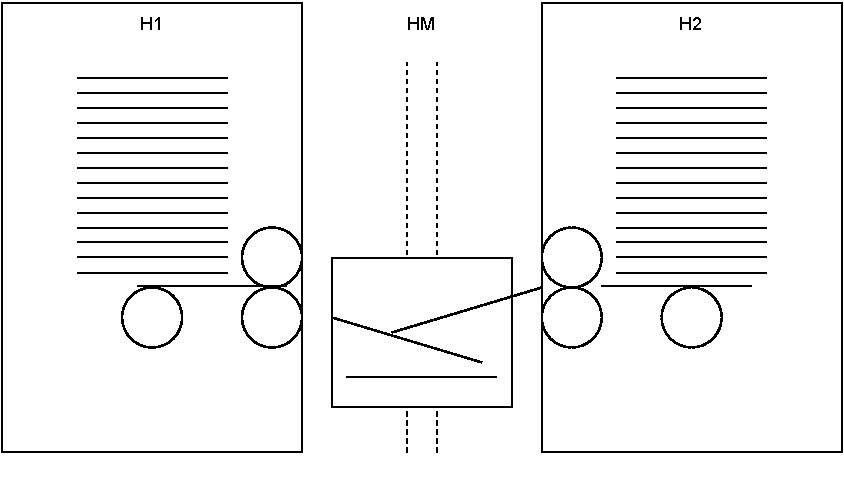
\includegraphics[width=0.9\linewidth]{irl_riffle_shuffle.pdf}
	\captionsetup{width=0.5\textwidth} \caption{Ett ilustrativt blandingsprocess
		diagram av
	Riffle Shuffle fundamentala mekaniska komponenter till den potentiella
	kortleksblandaren. Med 3 stycken högar $H1$, $HM$ respektive $H2$. Där sträckor representerar kort,
	cirkelformen representerar en roterande kortmatningsmekanism och mittersta
	högen är en höjbar mekanism i $y$-led.}
	\label{fig:irl_gsr}
\end{wrapfigure}

% \noindent
Första blandningsmetoden som anpassades var den matematiska
Gilbert-Shannon–Reeds modell till en praktisk Rust kod (för djupgående bakgrund
om modellen se sektion \ref{sec:riffle_shuffle}). För enkelhetens skull ska denna metod
betacknas \gls{gsr} Riffle Shuffle eller enbart \gls{gsr}. Motiveringen av att
utforska denna var  p.g.a. dess lockande egenskaper i att hur matematiska
modellen avspeglar människas kortblandningsprocess. Därför anpassades modellen för att
utforska om den kan vara ett lämligt kandidat till den potentiella
kortleksblandaren.

Matematiska formeln för \gls{gsr} distrubution är anpassad på rad 6 se Algoritm
\ref{alg:gsr}. För att inte distrahera med tekniska utmaningar implementation i
Rust finns i Bilaga \ref{app:gsr}.
% I implementeringen av detta algoritm inför simuleringen gjordes det några
% optimeringar som 1)  

\boldsection{Potentielt fysikt implementation}: Anpasnings metodiken av
\gls{gsr} inledes med att det skisades upp ett potentiell fysikt implementation av
Riffle Shuffle utifrån algoritmen, se Figur \ref{fig:irl_gsr}. Detta är ett
simplifierad version. För att t.ex. det borde finnas ett mekanism att flytta
kortet från $HM$ till $H1$ och $H2$. Kompliceringar i detta design kan inkludera
timing problem d.v.s. att kortet från $H1$ träffar kortet från $H2$ på vägen
till $HM$.

\begin{algorithm}
\caption{GSR Riffle Shuffle pseudokod}
\label{alg:gsr}
\begin{algorithmic}[1]
\State $H1 \gets$ $OD$ \Comment{Alla kort från $OD$ (Original Deck) är placerade i $H1$}
\State $H2 \gets \frac{H1}{2}$ \Comment{$H2$ får hälften av kort (i sekvensiell
ordining)}
\State $HM \gets tom lista$ \Comment{Mittersa högen}
\While{$H1$ eller $H2$ inte är tomma}
\State $r \gets$ slumpmässigt tal mellan 0.0 och 1.0 \Comment{\gls{prng} för att
få ett slumpmässigt tal}
    \If{$r \leq (\text{längden av } H1) / (\text{längden av } H1 + \text{längden av } H2)$}
        \State flytta ett kort från $H1$ till $HM$
    \Else
        \State flytta ett kort från $H2$ till $HM$
    \EndIf
\EndWhile
\State flytta alla kort från $HM$ tillbaka till $H1$
\end{algorithmic}
\end{algorithm}

\clearpage % To not weirdly wrap other text

 % Först att testa hur väl den utför till att avspegla hur en människa blandar
 % kort och att det krävs exakt 7 iterationer för en kortlekblanding att vara
 % slumpmässigt 
 % för att utforska hur väl den presterar i
 % kortleksblandingar och om den skulle vara en lämligt kandidat för den
 % potentiella kortleksblandaren.

\subsubsection{Anpassning av Pile Shuffle}
\begin{wrapfigure}{r}{0.6\textwidth}
% \begin{figure}[H]
	\centering
	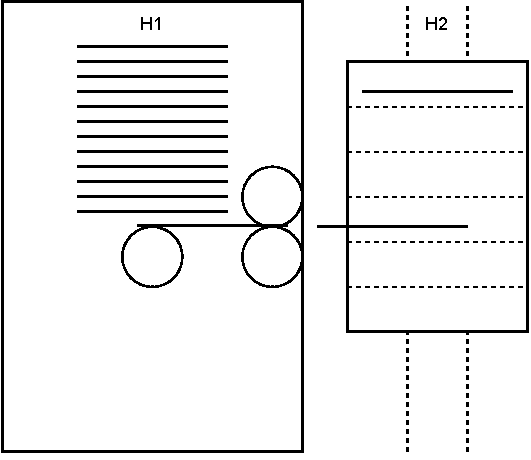
\includegraphics[width=0.6\linewidth]{irl_pile_shuffle.pdf}
	\captionsetup{width=0.5\textwidth} \caption{Ett ilustrativt diagram av
		kortblandningsprocesen med 
	Pile Shuffle metoden. Fundamentala mekaniska komponenter till den potentiella
	kortleksblandaren, där sträckor är kort, cirkelformen är roterande
kortmatningsmekanismen. Med två högar, $H1$ och $H2$. Där $H1$ har plats för en
kortlek medans $H2$ har $n$ antal fack med maximalt $M$ antal kort per fack.}
	\label{fig:irl_pile}
	
% \end{figure}
\end{wrapfigure}
Andra blandningsmetoden som anpassades var Pile Shuffle.
För det första är den metoden design mässig 
annorlunda till Riffle Shuffle. Den har endast en roterande
kortmatningsmekansim samt enbart två stora delar, se Figur
\ref{fig:irl_pile}. Insparation av det potentiella designen 
kom ifrån YouTube video 
\textcite{3DprintedLife2021}. I videon visas det en 3D printat kortleksblandare med Pile Shuffle algoritmen. Förkortningsvis denna  metod 
ska betecknas till \gls{soc} Pile Shuffle eller enbart 
\gls{soc}. Denna metod har två variarande inställningar som 
inkluderar 1) antal fack $n$ och 2) maximalt antal kort per
fack $M$. I denna studie utforskades både \gls{soc} samt 
två till variationer av denna Six Pile Shuffle respektive 
Ten Pile Shuffle. Med följande inställningar:
\textbf{\gls{soc} Pile Shuffle} med $n = 8$ och $M = 10$. Sedan utforskades hur påverkas slumpmässighet med färre fack
därmed fysiska designen kan vara mindre. Detta blev till 
algoritmen som betcknas till 
\textbf{Six Pile Shuffle} med $n = 6$ och $M = 10$. Sist undersöktes om vad sker om inställningar blir till $n = 10$ och $M = 10$ denna algoritm kallas till
\textbf{Ten Pile Shuffle}.

\begin{algorithm}
\caption{Pile Shuffle pseudokod}
\label{alg:pile}
\begin{algorithmic}[1]
\Require En kortlek $H1$
\Ensure Blandad kortlek $H1$ 
\State $n \gets num$ \Comment{Antal fack}
\State $M \gets num $ \Comment{Max antal kort per facket}
\State $H2 \gets$ lista av $n$ tomma listor % \Comment{Bins för korten}
\For{$kort$ i $H1$}
    \Loop
        \State $sf \gets$ slumpmässigt fack index mellan $0$ och ($n-1$) \Comment{slumpmässigt fack (sf)}
        \If{$\text{längden av } H2[sf] < M$}
            \State Lägg $kort$ i $H2[sf]$
            \State \textbf{break}
        \EndIf
    \EndLoop
\EndFor
\State $H1 \gets$ sammanfoga alla facken i $H2$ \Comment{Samla ihop alla fack till en kortlek}
\end{algorithmic}
\end{algorithm}


\subsubsection{Anpassning av design av professionell kortleksblandare}
Tredje blandningsmetoden som skapades var inspererad från en professionell
kortleksblandare. P.g.a. denna design har den fack för varje kort därmed anpassades det
Fisher-Yates Shuffle.
% (för detaljerna se sektion \ref{sec:fisher_yates}).
D.v.s. först blandades det en lista med indexes med
Fisher-Yates algoritmen och sedan kortet från $H1$ flyttas till $H2$ baserat på
slumpmässigt index se Figur \ref{fig:irl_wheel}. Detta metoden teoretiskt sätt
skulle kräva endast en iteration för att blanda en kortlek.

\begin{algorithm}
\caption{Wheel Fisher-Yates Shuffle pseudokod}
\label{alg:wheel}
\begin{algorithmic}[1]
\Require En kortlek $D$
\Ensure Blandad kortlek $D$ 
\State $I \gets$ lista med index $0$ till $51$ \Comment{Skapa en lista med index}
\State FisherYatesShuffle($I$) \Comment{Blanda indexen slumpmässigt}
\State $W \gets$ ny lista med $52$ platser \Comment{Skapa 'wheel' med plats för varje kort}
\For{$i \gets 0$ till $\text{längden av } D - 1$}
    \State $idx \gets I[i]$ \Comment{Välj ett slumpmässigt index från $I$}
    \State $W[idx] \gets D[i]$ \Comment{Placera kortet i 'wheel' baserat på slumpindex}
\EndFor
\State $D \gets W$ \Comment{Uppdatera $D$ med den nya ordningen från 'wheel'}
\end{algorithmic}
\end{algorithm}

% \begin{wrapfigure}{r}{0.6\textwidth}
\begin{figure}[H]
	\centering
	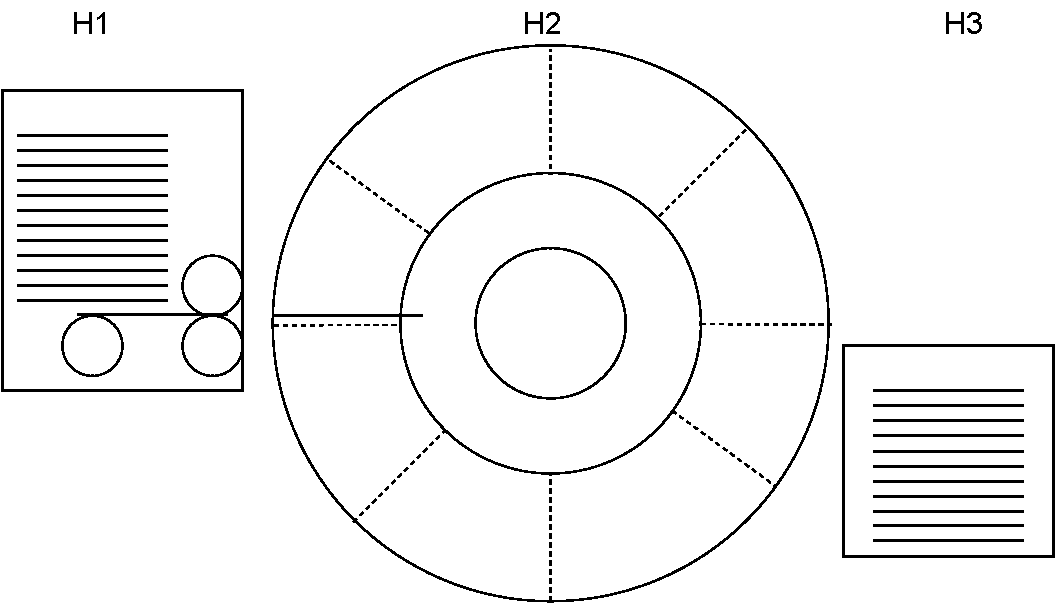
\includegraphics[width=0.6\linewidth]{irl_wheel_shuffle.pdf}
	\captionsetup{width=0.6\textwidth} \caption{Ett ilustrativt diagram av
		kortblandningsprocesen med 
	Fisher-Yates metoden. Fundamentala mekaniska komponenter till den potentiella
	kortleksblandaren, där sträck är kort, cirkelformen är roterande
kortmatningsmekanismen. Med två högar, $H1$ och $H3$. Där $H2$ har ett fack för
varje kort, d.v.s. 52 stycken. Och $H3$ är plats till en blandad kortlek.}
	\label{fig:irl_wheel}
\end{figure}
% \end{wrapfigure}
% \noindent

% \clearpage

\subsection{Simulering av kortblandningsprocesser}
\label{sec:sim_kort}
Simulations- och blandningsalgoritmerna implementerades i programmerings språk
Rust version 1.73.0. Rust valdes p.g.a dess robusta stöd för abstraktioner utan bekostnad.  
% Datan insamlades från digitalt simulation på olika kortblandningsmetoder
% i Rust version 1.73. De algoritmerna som undersöktes var skrivna i
% programspråk Rust i försök att göra dem så likt verkligheten som
% möjligt. 

% \lstinputlisting[language=Python, caption={Pile Shuffle skriven i
% Rust},label=selection-sort, label={lst:algo_2},firstline=329,
% lastline=335]{../randomness/sim_stats.py}

% För statistikst analys av data användes programmeringsspråket Python
% 3.11 och utnyttjades bibliotek som Numpy till datamängd bearbetning,
% Scipy till statistisk analys och Matplotlib till visualisering av
% resultat. 

% Den Valdes på grund av dess breda användning inom vetenskapligt
% forskning  och dess omfattande bibliotek för numerisk analys.  

% och användes bibliotek (Rust Crates) som Rand version 0.8 för PRNG
% \parencite{rand_crate}. Rayon för enkel användning av  parallell
% multiprocessing
% \parencite{rayon_crate}.
Simulationen avspeglar hur ett fysiskt kortleksblandare skulle fungera. Därför
togs det valet att alla simulationer ska ha ett och samma utgångspunkt. Därmed i
analysen kan det jämföras olika metoder beroende på deras iterationer. D.v.s. ett verkligt
scenarium simulerades vart ett helt ny oöppnad kortlek skulle placeras i den
potentiella kortleksblandare. Detta ordningen kallas för ett fabriksordning för
en standard 52-kortlek. Där korterna är ordnade efter sitt färg i sekvensiell
ordning från två till ess (utan jokrarna). Matematiskt kan detta ordningen
beskrivas som mängden $\{x \in \mathbb{N},  0 \leq x \leq 51 \}$, där $x$
representerar en enskild kort och vart ordningen spelar roll. 

För att bestäma datamängden d.v.s. antal kortlekar per en simulation. Användes
det rekomendationen för chi-två-testet. Där NIST rådger att minsta förekommande
kategorin för pokertest borde inte vara mindre än 5 stycken (se sektion
\ref{sec:chi_square}). 
% Simulation utgår från att man genererar
% tvådimmensionella array, detta kan matematikst beskrivas som matris med
% bestämd mängd av kortlekar. Vart varje kort, låt kalla dem till $x$ som
% följer följande mängden $\{x \in \mathbb{N},  0 \leq x \leq 51 \}$
% Resulterande datamängden är en \gls{matris} $D$ med 52 kolumner och $m$ antal
% rader, vart $m$ värde visar hur många kortlekar det finns i datamängden.
% För att bestämma värdet för $m$ följdes ett kriterium ifrån klassiskt
% poker test (mer i  detalj beskriven i underrubriken
% \ref{sec:chi_square}).
% Till hjälps användes NIST internätkälla   i
% denna nämns det att det är viktigt för chi-square approximationens trovärdighet
% att minsta kategorin ska inte vara mindre än fem teoretiska framkommande i den
% kategorin \parencite{nist}. Därför är det
% viktigt att hitta den minsta kategorin som kan förekomma.
I poker är den mest
sällsynta pokerhanden den kungliga färgstegen (Royal Flush) och det finns 4
stycken av dessa i en standardkortlek. Den teoretiska sannolikheten att
få 5 Royal Flushes per $m$ kortdelnigar kan aproximeras på följande sätt: 
% som kan räknas ut på
% följande sätt antal av alla kortkombinationer med fem kort. $\binom{52}{5} =
% 2\,598\,960$ Kungliga färgstege finns det fyra  kombinationer av i kortleken
% som kan räknas ut på följande sätt totala antal kombinationer av kungliga
% färgstege delat med totala antal femkorts kombinationer från standardkortlek.
$$ P(\text{Kunglig färgstege}) =  \frac{\binom{4}{1}}{\binom{52}{5}} =
\frac{4}{2\,598\,960} \approx \frac{1}{649\,740} $$ 
Sedan denna  resultatet skalas med faktor av 5:
$m = P(\text{Kunglig färgstege})^{-1}  \times 5 = 3\,248\,700$.
Denna resulterande värden på $m$ används som den absoluta längden av datamängden i
simulationen. För att visualisera detta, låt $D$ vara en \gls{matris} 
med 52 kolumner (antal kort i standardkortleken) och $m$ antal rader (längden av
datamänden), och där $x$ är en av talen ur den tidigare definerade mängden.
\begin{equation*}
	D = \begin{bmatrix}
		x_{0,0} & x_{0,1} & x_{0,2} & \cdots & x_{0,51}\\ 
		x_{1,0} & x_{1,1} & x_{1,2} & \cdots & x_{1,51}\\
		x_{2,0} & x_{2,1} & x_{2,2} & \cdots & x_{2,51}\\
		\vdots & \vdots & \vdots & \; & \vdots \\
		x_{m,0} & x_{m,1} & x_{m,2} & \cdots & x_{m,51}
	\end{bmatrix}
\end{equation*}

% \subsubsection{Val av datatyp \& rådatalagring} 

% Efter teoretiska beräkningar av
% datamängden är det viktigt att välja en lämplig datatyp att representera data i.
% Högsta talet som behövs är 51 definerad tidigare och betecknat med $x$. Detta
% betyder att den minsta datatypen som får användas är 8 bit eller 1 byte långa som
% kan  innehålla följande värden $$\{b \in \mathbb{N},  0 \leq b \leq 255 \}$$ som
% överns\-stämmer med datamängdens högsta talet $x$. Detta ger möjligheten att
% använda den  fundermantala datatypen som används i minnesadressen. Fördelen med
% detta är det simplifierar lagring och inmatning av datamängder i t.ex Python
% med NumPy.
Via expermintell metodik valdes det att utföra 15 iterationer
per algoritm. En iteration defineras till att kortleken blandas successiv på
föregånde blandning. Detta gjordes 
för att senare kunna jämföra hur algoritmens slumpmässighet påverkas av ökande 
antal iterationer. Dessutom kan detta valet motiveras av att \gls{gsr}s matematiska
modellen visar sig att vara mest effektiv vid 7 och 11 iterationer (se sektion
\ref{sec:riffle_shuffle}). Detta antal iterationer kunde
ske p.g.a att simulationsprocessen effektiviserades med Rayon \gls{crate}.
% simulationen 
Med denna verktyg utfördes programmet i parallelt exekvering. 
% På ett
% effektivt sätt simulerades det mer data.
% Detta valet
% togs för att algoritmerna är oberoende av varandra.
% och att på detta sättet
% .  
% Därfor mer iterationer utfördes och
% på så sätt mer data insamlades.
% Därför infördes
% det 4 iterationer till för mer analysdata.

För att förutspå hur mycket RAM och hårddisk minne  skulle eventuellt användas vid
lagring och datanalys. Räknades det ut tynged av en datamängd ska väga 
% Där ett kort är representerat i uint8
% (8-bit lång datatyp)
% användes. Tynged av datan räknades till
% Andra aspekten till varför datatypen är viktigt är att spara minnen för att det
% kommer att simuleras och sparas tiotals rådata filer varje fil kommer att väga
$161 MB$ vid använding av 8bit datatypen.
$$ \frac{\text{totala bytes}}{\text{megabyte (MB)}} = \frac{52 \times m }{1024 \times
1024} = \frac{52 \times 3\,248\,700}{1024 \times 1024} = \frac{168\,932\,400}{1\,048\,576} \approx 161 MB 
$$
Detta steget behövdes för att ta ett informativ beslut senare. D.v.s. hur data ska
analysers och eventuella anpassas.
% och proccessen effektiviseras.   

Som det tidagare nämndes utfördes simulationen parallelt där varje algoritm
exekverades på egen tråd, oberoende av varandra.
Simulationen utfördes i följande steg: 
1) Algoritmenerna sparades i en lista;
2) En lista av kortlekar, motsvarande matrisen $D$ med $m$ antal kortlekar, initierades till fabriksordningen; 
3) Algoritmerna itererades i en nästlad loop från $i = 1$ till $i = 15$; 
4) Ledtidsmätaren sätts igång;
5) Denna iteratinsvariabel $i$ användes för att iterera över listan av kortlekar
och utföra blandningen $i$ gånger;
6) Efter varje iteration $i$ adderades ledtiden;
7) Efter avklarad iteration $i$ medelvärde av ledtiden kalkylerades och
sparades i en csv fil;
8) Resulterande blandade kortlekarna utplattedes till en endimensionell lista;
9) Denna endimensionella lista sparades som en binärfil för statistiskanalys.

% som det är enkelt att spara data i binärt format för att 8 bits eller 1 byte
% är ett fundamentalt och uniformt mått i minnesadressen. Med det sagt, ingen
% bearbetning av data behövs och det är enkelt att ladda in denna i till exempel Python
% med numpy till statistiska testerna av rådata
%
% Därför att sista teoretiska delen att bestämma
% är hur många iterationer per algoritm ska genomföras. Med iterationer menas
% hur många gånger kortleken blandas följande på varandra.


\subsection{Statistisk analys av insamlad data.}
Detta sektion handlar om hur statistiska metoder som Poker test och
\gls{stdmean} test implementerades för att analyser slumpmässighet av valda och
simulerade algoritmerna. Statistiska tester utfördes med Python version 3.11.
Python valdes p.g.a dens breda använding vid statistisk analys (se sektion
\ref{sec:verktyg}).

Efter simulationen, insamlad data är laddat in och återställt tillbaka till
formen av matrisen $D$ från sektion \ref{sec:sim_kort} med hjälp av NumPy för vidare
bearbetning. Analysmetoderna delar inladdat data p.g.a. optimeringskall som e.g.
spara minnen och minimisera initial exekveringstid.

På grund av begränsad kunskap och expertis inom avancerad statistisk matematik,
även om metoder såsom Aproximate Entropi (\gls{apen}) skulle kunna erbjuda
ytterligare insikter i slumpmässighetsanalys \parencite{ApEn}, valdes det att
inte använda dem i denna studie. Detta beslut baserades på bristen på fördjupade
kunskaper inom detta område samt tidsbegränsingen. Istället fokus ligger på en
annan branch av slumpmässighet baserad på
sannolikhetslära. % (se \ref{sec:slump})

% områden inom matematiken som statistikt analys. Detta betyder att rent
% matematiska modeller till avgörande av slumpmässighet som approximate
% entropi (\gls{apen})   Men den 

% Men för att avgörande av
% slumpmässighet är domän specifikt och rent matematiskt komplex då krävs
% det högre förstålse i matematatikens området inom statistik.  Istället
% valdes det att fokuser på normal distrabition av kortlekar och kort.
% Dessutom implementerades det metoder som är visuellt representativa.

% Från
% andra sidan är simulation enklare att utföra och analysera data med
% avseende på förväntade frekvensen ($\chi^2$-testet) samt enklare
% statistiska koncept som mediana och standardavviklse (StdMean-testet).


% För statistikst analys av data användes programmeringsspråket Python
% 3.11 och utnyttjades bibliotek som Numpy till datamängd bearbetning,
% Scipy till statistisk analys och Matplotlib till visualisering av
% resultat. 

% med följande
% metoder: Klassisk Poker Test \ref{sec:poker_test} och medelvärde av
% korta positioner i kortleken över hela datamängden kalkylerad såsom
% avvikelser av dessa positioner. Utförligt beskrivning i underrubriker. 

\subsubsection{Implemention av den klassiska poker testet}
Syfte med denna metod är att utföra preliminär galring av algoritmernas
iterationer som har betyande avvikelser från dem förväntade värdena av en slumpmässigt
blandningsalgoritm.  

Den klassiska poker test utgår ifrån att man karaktäriserar typer av mönster
till pokerhänder och kalkylerar  den absolut värde av $\chi^2$ i detalj beskrevs
teorin bakom chi-två-test  i sektion \ref{sec:poker_test}. Den klassiska poker
testet i denna studie baseras på faktumet att simuleringar utfördes med en
standard kortlek. Därför valdes det att anpassa chi-två-testet att använda alla
poker händer. Matematiken, speciellt kombinatoriken att räkna ut sannolikheter
och frekvensen av alla poker\- händer är relativt svår uppdrag därför
addopterdes det uträkningar ifrån studie av \textcite{Drew2006}, se tabell
\ref{tab:all_poker_hands}. Detta metodiken medföljde med mer komplex
karakterisering av poker\-händer än när man använder chi-två-testet till att
e.g. testa slumptalsgeneratorer. Motiveringen till komplixiteten var att i denna
studie utforskas särkilt kortlekar till spel vart kombinationer av kort ofta
spelar betyande roll och därför var det särkilt viktigt att anpassa
slumpmässighets analysmetoderna till hur den potentiella kortleksblandare skulle
fungera i drift.

\begin{table}[H] 
\captionsetup{width=0.5\textwidth, justification=centering}
\caption{Namn på alla pokerhänder och dess relativ mönster. Antal$_1$ är 
teoretisk framkommande kombinationer med en standard kortlek. Antal$_2$ är 
faktoriserade kombinationer d.v.s \\ Antal$_2 = $ Antal$_1 \times 1.25$ }
\label{tab:all_poker_hands}
	\centering
	\begin{tabular}{|l|c|r|r|}
	
	% Header
	\hline 
	Pokerhand 
	& Example mönstren 
	& Antal$_1$ 
	& Antal$_2$ 
	\\ \hline  

	% rows
	Royal Flush 
	& $A\spadesuit\, K\spadesuit\, Q\spadesuit\, J\spadesuit\, 10\spadesuit$
	& 4 
	& 5
	\\ \hline

	Färgstege
	& $K\spadesuit\, Q\spadesuit\, J\spadesuit\, 10\spadesuit\, 9\spadesuit$
	& 36 
	& 45
	\\ \hline

	Fyrtal 
	& $A\spadesuit\,A\heartsuit\,A\diamondsuit\,A\clubsuit\, K\spadesuit$ 
	& 624 
	& 780
	\\ \hline

	Kåk 
	& $A\spadesuit\, A\heartsuit\, A\diamondsuit\, K\clubsuit\,K\spadesuit$ 
	& 3\,744
	& 4\,680
	\\ \hline

	Färg
	& $K\spadesuit\, Q\spadesuit\, J\spadesuit, 10\spadesuit\, 8\spadesuit$
	& 5\,108
	& 6\,385
	\\ \hline

	Stege 
	& $K\spadesuit\, Q\heartsuit\, J\diamondsuit\, 10\clubsuit\,9\spadesuit$ 
	& 10\,200
	& 12\,750
	\\ \hline
	Triss 
	& $A\spadesuit\, A\heartsuit\, A\diamondsuit\, K\clubsuit\, Q\spadesuit$
	& 54\,912
	& 68\,640
	\\ \hline

	Två par 
	& $A\spadesuit\, A\heartsuit\, K\diamondsuit\, K\clubsuit\, Q\spadesuit$
	& 123\,552
	& 154\,440
	\\ \hline

	Ett par 
	& $A\spadesuit\, A\heartsuit, K\diamondsuit\, Q\clubsuit\, J\spadesuit$ 
	& 1\,098\,240 
	& 1\,372\,800
	\\ \hline

	Högt kort
	& $A\spadesuit\, Q\heartsuit\, J\diamondsuit\, 5\clubsuit\, 4\spadesuit$
	& 1\,302\,540
	& 1\,628\,175
	\\ \hline

	 
	\multicolumn{2}{|r|}{Summan:} 
	& 2\,598\,960 
	& 3\,248\,700
	\\ \hline
\end{tabular}
\end{table}

\noindent
Kategeriseringsprocessen till att få ett hand till ett pokerhand börjades med
att det uttnytjades NumPy vektoriserad aritmetik funktionalitet. Med denna
funktionen på ett effektivt sätt valdes ut 5 kort i.e en hand och kördes igenom
en katigoriserings funktion om denna senare. Dem 5 kort valdes ut på ett
speciellt sätt för att göra denna likvärdig verkligheten. D.v.s. pokerspel med 2
spelare. Där valdes det kort med index 0, 2, 5, 6 och 7 (spelare-ett:  2 kort i
handen, spelare-2 kort förkastas och 3 sista kort är flop) med NumPy funktionalitet
kördes katigoriserings funktionen rad mässigt.

\textbf{katigoriserings funktion:}
I standardkortlek finns det 52 kort med fyra olika 
färger (Spader, Hjärter, Ruter och klöver) och 13 valörer 
(2, 3, 4, 5, 6, 7, 8, 9, 10, Knekt, Dam, Kung, Ess). Konvertering av tidigare
definerade mängden av kort $x$, i.e. (0, 1, 2, $\dots$, 51) till katgeriserbart
kort utfördes. För att optimera kategoriseringsproccessen användes Numba för att skapa en
ny tråd, detta kunde enbart göras p.g.a. att det användes den fundamentala 8bit
datatypen, som definerades tidigare. Efter att ett ny tråd skapades proccessen
försattes på följande sätt: 
\begin{equation*}
    \text{valör}(x) = x \mod 13
\end{equation*}
\begin{equation*}
    \text{färg}(x) = \left\lfloor \frac{x}{13} \right\rfloor
\end{equation*}
där $\text{valör}(x)$ ger värde från 0-12 och $\text{färg}(x)$ ger värde från
0-3. För dem intresserade av specifika kod detaljerna se Bilaga
\ref{app:github}. Försättningsvis denna funktion gav tillbaka ett värde från
0-9 som indikerar ett pokerhand ifrån Tabell \ref{tab:all_poker_hands}, där 0 är
Högt kort och 9 Royal Flush. För att denna funktionen kördes kolumn mässigt över
hela datamängded var denna resulterande 
lista med antal observerade pokerhänder från varje rad, låt denna lista betecknas till
$O$ (Observerat frekvens). I bästa fall skulle denna lista
fått likadana värdena som kolumnen Antal$_2$ i Tabell \ref{tab:all_poker_hands}.


\textbf{Chi-två-test}: Inställningar till testet var $\alpha = 0.05$
(\gls{alfa}), df $= 10 -
1 = 9$ (frihetsgrader), där $10$ är den antal pokerhänder givna av Tabell
\ref{tab:all_poker_hands}. Sedan beräknades gränsvärde med SciPy \gls{bibliotek}s
funktionen $Chi2.ppf( 1 - \alpha, df)$. Sedan används det \textit{chisquare}
funktionen ifrån SciPy för att beräkna \gls{pvalue} och $\chi^2$ värde. För att
kalkylera denna användes tidigare genererade listan $O$ och dem förväntade värden given av
kolumnen Antal$_2$ i Tabell \ref{tab:all_poker_hands}. Resulterande värdena på
\gls{pvalue} och $\chi^2$ sparades i en csv fil för redovisningen i Resultat
sektionen.

\subsubsection{Implemention av STDMean testet}
Syfte med denna analysmetod är att utforska hur enskild kort rör sig genom
kortleken när den blandas. Därmed avgöra om algoritmen har eller har inte ett
tendens att blanda specifika delar av kortleken mer än dem andra. Detta i sin
tur är viktigt i kortspel där positioner på första korterna är viktiga för
kortspels rätvisshet. Snedvridning kan alltså potentiell indikera logiska fell i
implementionen av en algoritm. I initiala tester användes \gls{stdmean} testet
för att upptäcka logiska fel. Detta hände i den första versionen av
implementation av \gls{gsr} Riffle Shuffle, där det på fell sätt användes indexering
i iterationen, felet upptäcktes med hjälp av denna analysmetoden. 

För att förstå metoden är det relevant att återbesöka konceptet med matrisen $D$ i sektion 
\ref{sec:sim_kort}. Därför att det uttnytjade NumPy vektoriserad aritmetik i
simbios med dens inbyggda funktioner som medelvärde och standardavvikelse. Både
funktionera utfärdes kolumn vis på $m$ antal rader. Denna resultatet användes sedan till
att rita punktdiagram av Medelvärde av Position på y-led (\gls{mp}) och
Position av Kort på x-led (\gls{pk}). Standardavviklse från medelvärdet visas
som symetrisk linje ifrån denna punkten. Den teoretiska medelvärdet i 
en slumpmässigt blanding borde ligga runt $51 \div 2 = 25.5$ och den
experimentellt testade standardavvikelse ifrån medelvärdet $\approx 15$.

\section{Resultat}
% Result är icke bestämt i vilken format kommer att skrivas
% Men dem kommer att innehålla figur \ref{fig:test_figure}. Antagligen mest 
%intresanta figurer kommer att visas här och alla andra Bilagas i Appendix.
%För att det kommer att vara minst 30 figurer och chi två tabeller(dem 
%kan göras i ett större tabell, antar jag)


Totalt 75 simulationer av olika kortblandnings algoritmer utfördes. 15
simulationer per algoritm för att jämföra samma algoritm med olika antal
iterationer, varje algoritm har alltså resultat som motsvarar utförelse
med iterationer 1-15. Dem viktigaste av simulationerna plockades ut och
deras resultat presenteras här. Resultat av poker test samt medelvärde
för algoritmers ledtid presenteras i tabeller. Resultaten för medelvärde
av dem positioner ett kort har varit på och standardavvikelsen
presenteras via punktdiagram. Vilket kort som en punkt i diagrammet
representerar ges av punktes position på x-axeln, medelvärde är avläst
från punktens position på y-axeln och standardavvikelse är givet av
linjen som går genom punkten. 

\begin{table}[H]
	\centering
	\captionsetup{width=0.5\textwidth}
	\caption{Resultatet från det klassiska pokertestet: Gränsvärde
	fastställt till 16.92 vid en signifikansnivå (\(\alpha\)) på
	0.05 och med 9 frihetsgrader (df). Vart ledtiden representerar
	medelvärdet för en kortleksblandning per iteration.}

	\label{tab:res-pokertest}
	\begin{subtable}[h]{0.45\textwidth}
		\centering
		\caption{\gls{gsr} Riffle Shuffle}
		\label{tab:gsr}
		\begin{tabular}{c|c|c|c}
			%\hline
			$\phantom{\bigg|}$ Iteration & $\chi^2$  & \(p\)-värde & Ledtid [ns]
			\\ \hline \hline
			3 & 233941.28 & 0 & 1681
			\\ \hline 
			4 & 7077.30 & 0 & 1687 
			\\ \hline
			5 & 449.67 & 3.38 & 1660 
			\\ \hline
			6 & 34.46 & 7.42 & 1667
			\\ \hline
			7 & 6.03 & 0.74 & 1654 
			\\ \hline
			8 & 8.50 & 0.48 & 1642 
			\\ \hline
			9 & 19.64 & 0.020 & 1582 
			\\ \hline
			10 & 8.88 & 0.45 & 1495 
			\\ \hline
			11 & 16.19 & 0.063 & 1432 
		\end{tabular}
	\end{subtable}
	\hfill
	\begin{subtable}[h]{0.45\textwidth}
		\centering
		\caption{Six Pile Shuffle}
		\label{tab:six}
		\begin{tabular}{c|c|c|c}
			$\phantom{\bigg|}$ Iteration & $\chi^2$  & \(p\)-värde & Ledtid [ns]

			\\ \hline \hline
			1 & 3854.97 & 0 & 1116 
			\\ \hline
			2 & 18.36 & 0.031 & 1124 
			\\ \hline
			3 & 12.27 & 0.20 & 1131
			\\ \hline
			4 & 5.94 & 0.75 & 1184 
			\\ \hline
			5 & 12.34 & 0.19 & 1167 
			\\ \hline
			6 & 8.89 & 0.45 & 1168 
			\\ \hline
			7 & 4.33 & 0.89 & 1211 
		\end{tabular}
	\end{subtable}

	\vspace{2em}

	\begin{subtable}[h]{0.45\textwidth}
		\centering
		\caption{\gls{soc} Pile Shuffle}
		\label{tab:soc}
		\begin{tabular}{c|c|c|c}
			$\phantom{\bigg|}$ Iteration & $\chi^2$  & \(p\)-värde & Ledtid [ns]

			\\ \hline \hline
			1 & 3349.24 & 0 & 1450 
			\\ \hline
			2 & 7.02 & 0.64 & 1465 
			\\ \hline
			3 & 19.11 & 0.024 & 1518
			\\ \hline
			4 & 7.53 & 0.58 & 1441 
			\\ \hline
			5 & 8.50 & 0.48 & 1501 
			\\ \hline
			6 & 12.34 & 0.19 & 1536 
			\\ \hline
			7 & 8.36 & 0.50 & 1577 
		\end{tabular}
	\end{subtable}
	\hfill
	\begin{subtable}[h]{0.45\textwidth}
		\centering
		\caption{Ten Pile Shuffle}
		\label{tab:ten}
		\begin{tabular}{c|c|c|c}
			$\phantom{\bigg|}$ Iteration & $\chi^2$  & \(p\)-värde & Ledtid [ns]

			\\ \hline \hline
			1 & 3349.24 & 0 & 1587 
			\\ \hline
			2 & 5.83 & 0.76 & 1654 
			\\ \hline
			3 & 4.83 & 0.85 & 1716
			\\ \hline
			4 & 5.38 & 0.80 & 1625 
			\\ \hline
			5 & 5.09 & 0.82 & 1697 
			\\ \hline
			6 & 8.80 & 0.46 & 1698 
			\\ \hline
			7 & 14.46 & 0.11 & 1710 
		\end{tabular}
	\end{subtable}
	\vspace{2em}

	\begin{subtable}[h]{0.45\textwidth}
		\centering
		\caption{Wheel Fisher-Yates Shuffle}
		\label{tab:wheel}
		\begin{tabular}{c|c|c|c}
			$\phantom{\bigg|}$ Iteration & $\chi^2$  & \(p\)-värde & Ledtid [ns]

			\\ \hline \hline
			1 & 10.71 & 0.30 & 715 
			\\ \hline
			2 & 13.46 & 0.14 & 720 
			\\ \hline
			3 & 6.66 & 0.67 & 728
			\\ \hline
			4 & 9.05 & 0.43 & 733 
			\\ \hline
			5 & 8.95 & 0.44 & 772 
			\\ \hline
			6 & 6.10 & 0.73 & 794 
			\\ \hline
			7 & 9.41 & 0.40 & 778 
		\end{tabular}
	\end{subtable}
\end{table}

\begin{figure}[H]
	\centering
	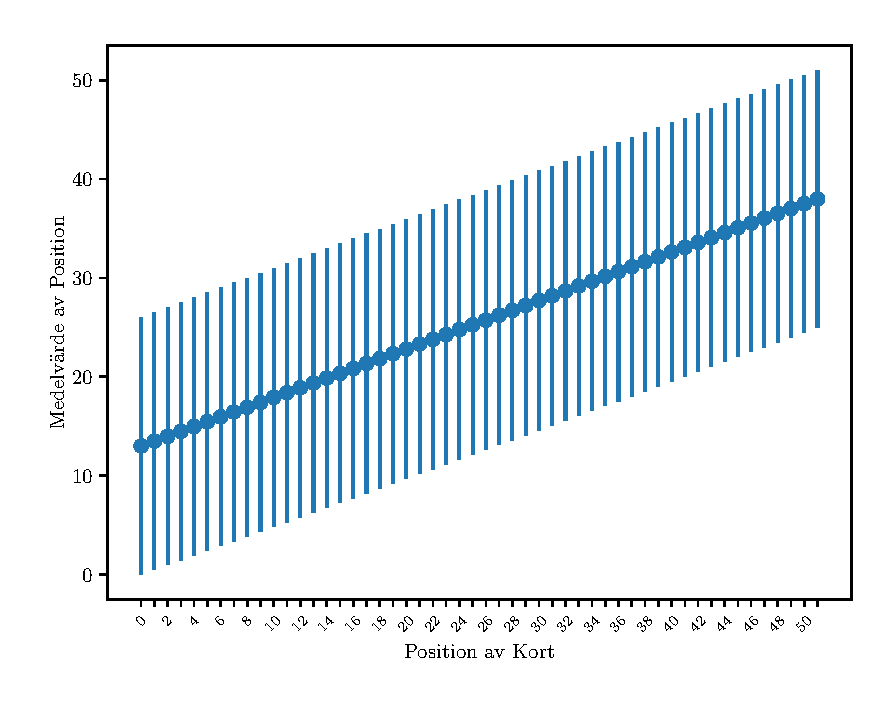
\includegraphics[width=0.8\textwidth, trim={0.8cm 0.8cm
	0.75cm 0.75cm}, clip]{gsr_riffle_shuffle-1}
	\captionsetup{width=0.5\textwidth}
	\caption{Resultatet från \gls{stdmean} testet  för \gls{gsr}
	Riffle Shuffle med \textbf{1} iteration.}
	\label{fig:gsr-1}
\end{figure}

\begin{figure}[H]
	\centering
	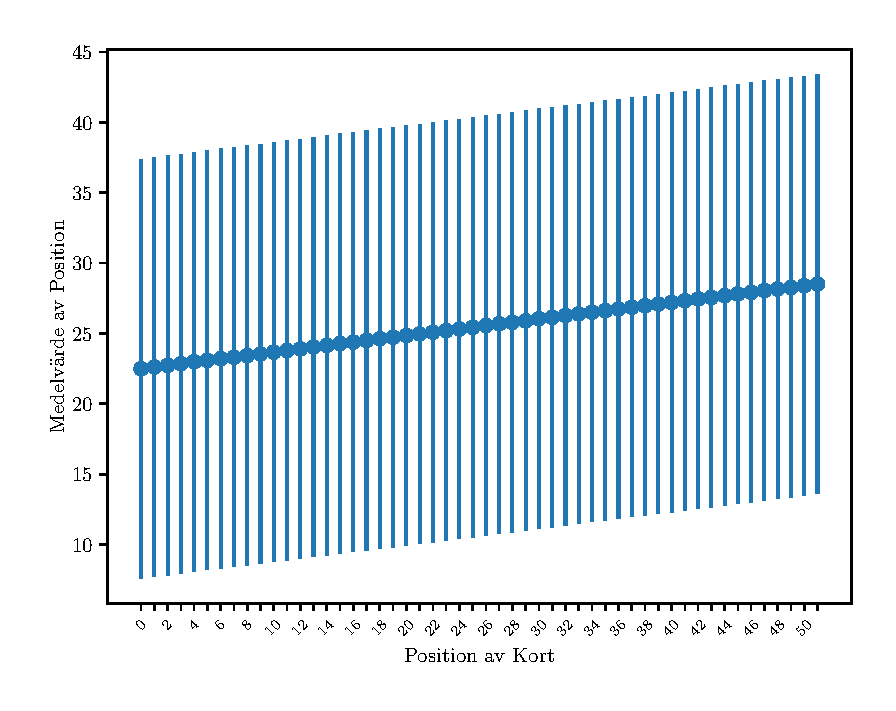
\includegraphics[width=0.8\textwidth, trim={0.8cm 0.8cm
	0.75cm 0.75cm}, clip]{gsr_riffle_shuffle-3} 
	\captionsetup{width=0.5\textwidth}
	\caption{Resultatet från \gls{stdmean} testet  för \gls{gsr}
	Riffle Shuffle med \textbf{3} iterationer.}
	\label{fig:gsr-3}
\end{figure}

\begin{figure}[H]
	\centering
	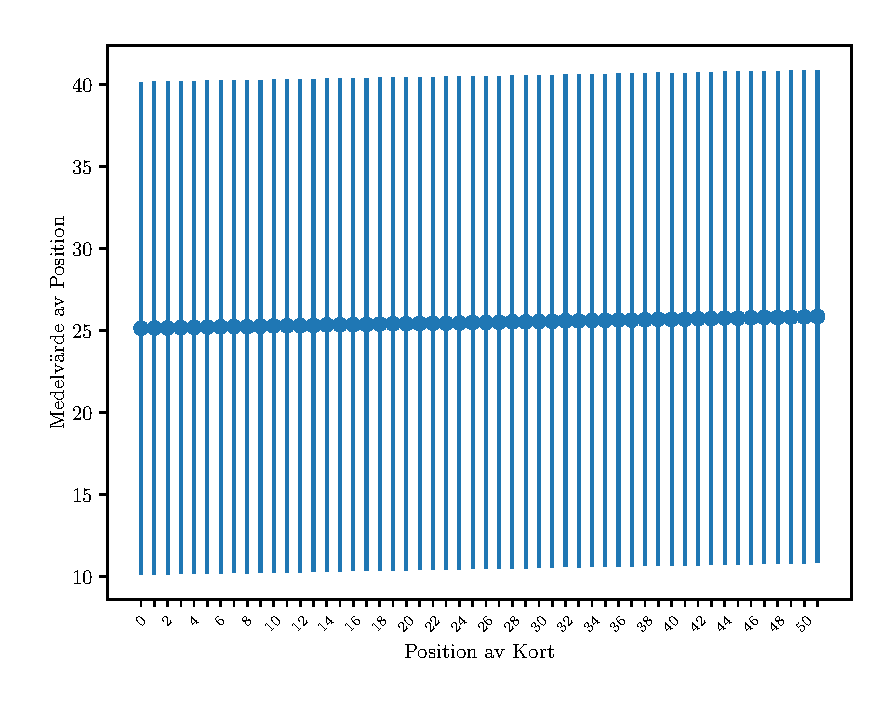
\includegraphics[width=0.8\textwidth, trim={0.8cm 0.8cm
	0.75cm 0.75cm}, clip]{gsr_riffle_shuffle-6} 
	\captionsetup{width=0.5\textwidth}
	\caption{Resultatet från \gls{stdmean} testet  för \gls{gsr} Riffle
	Shuffle med \textbf{6} iterationer.}
	\label{fig:gsr-6}
\end{figure}

\begin{figure}[H]
	\centering
	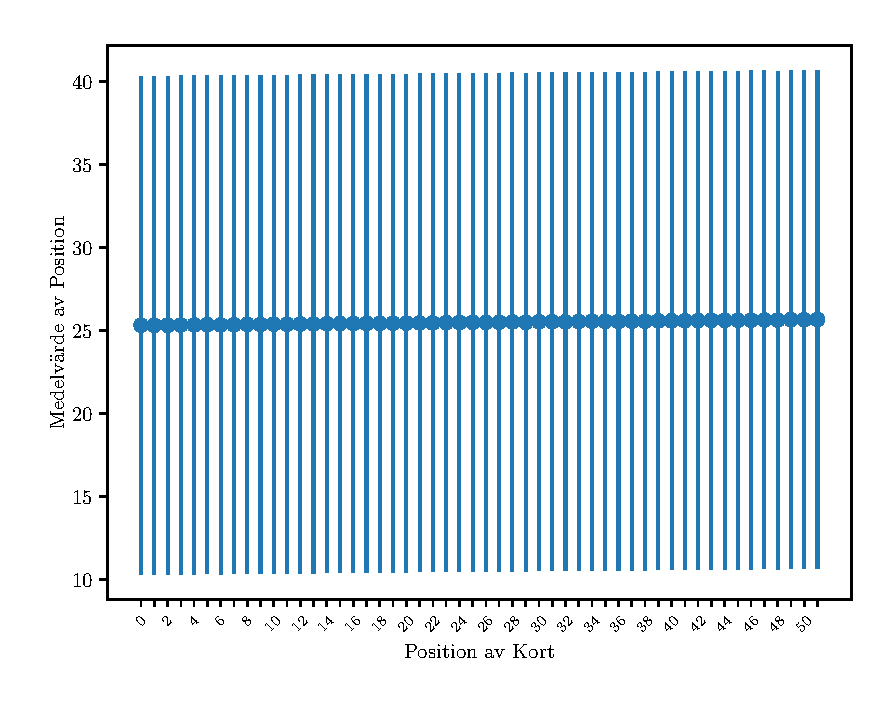
\includegraphics[width=0.8\textwidth, trim={0.8cm 0.8cm
	0.75cm 0.75cm}, clip]{gsr_riffle_shuffle-7} 
	\captionsetup{width=0.5\textwidth}
	\caption{Resultatet från \gls{stdmean} testet för \gls{gsr} Riffle Shuffle
	med \textbf{7} iterationer.}
	\label{fig:gsr-7}
\end{figure}

\begin{figure}[H]
	\centering
	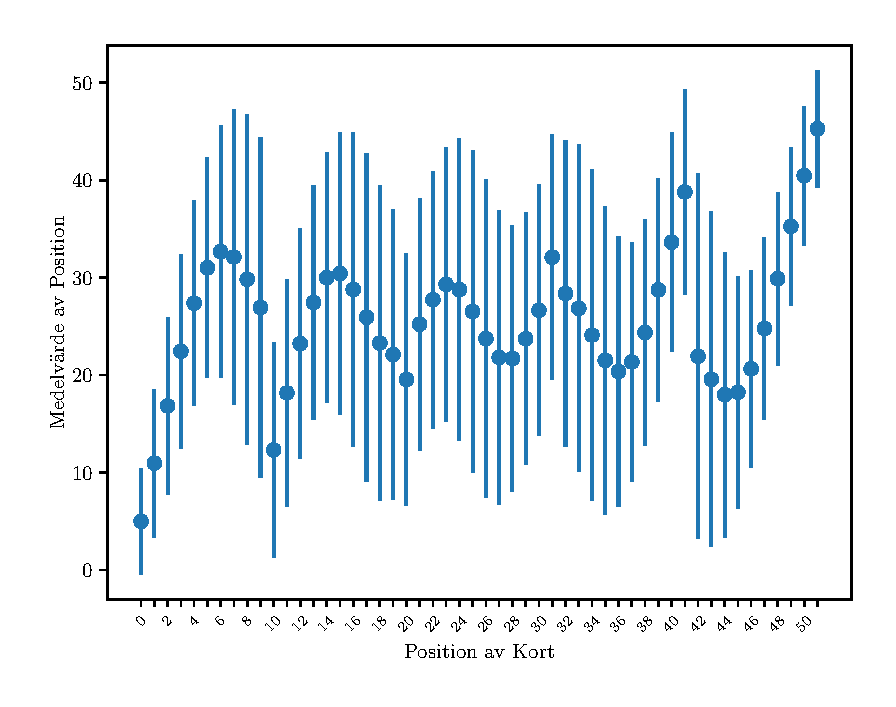
\includegraphics[width=0.8\textwidth, trim={0.8cm 0.8cm
	0.75cm 0.75cm}, clip]{six_pile_shuffle-1} 
	\captionsetup{width=0.5\textwidth}
	\caption{Resultatet från \gls{stdmean} testet för Six Pile
	Shuffle med \textbf{1} iterationer.}
	\label{fig:six-1}
\end{figure}

\begin{figure}[H]
	\centering
	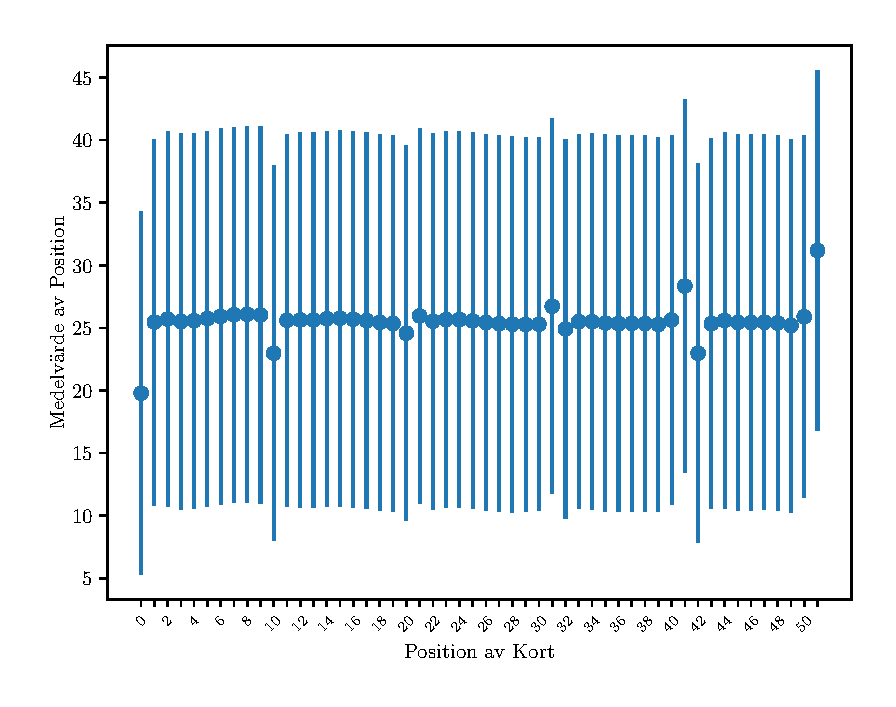
\includegraphics[width=0.8\textwidth, trim={0.8cm 0.8cm
	0.75cm 0.75cm}, clip]{six_pile_shuffle-2} 
	\captionsetup{width=0.5\textwidth}
	\caption{Resultatet från \gls{stdmean} testet för Six Pile
	Shuffle med \textbf{2} iterationer.}
	\label{fig:six-2}
\end{figure}

\begin{figure}[H]
	\centering
	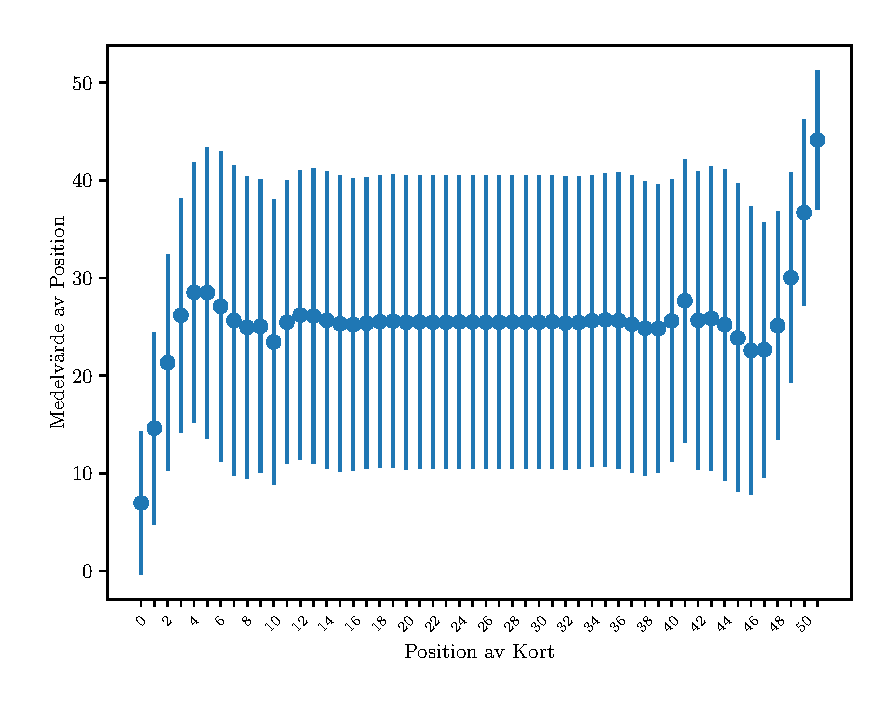
\includegraphics[width=0.8\textwidth, trim={0.8cm 0.8cm
	0.75cm 0.75cm}, clip]{soc_pile_shuffle-1} 
	\captionsetup{width=0.5\textwidth}
	\caption{Resultatet från \gls{stdmean} testet för \gls{soc} Pile
	Shuffle med \textbf{1} iteration.}
	\label{fig:soc-1}
\end{figure}

\begin{figure}[H]
	\centering
	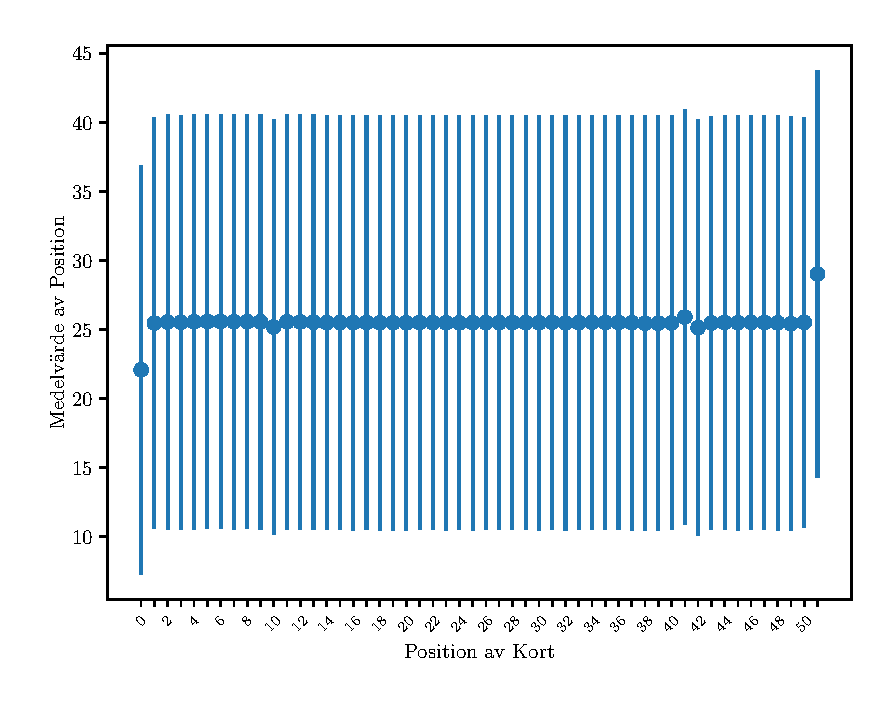
\includegraphics[width=0.8\textwidth, trim={0.8cm 0.8cm
	0.75cm 0.75cm}, clip]{soc_pile_shuffle-2} 
	\captionsetup{width=0.5\textwidth}
	\caption{Resultatet från \gls{stdmean} testet för \gls{soc} Pile
	Shuffle med \textbf{2} iterationer.}
	\label{fig:soc-2}
\end{figure}

\begin{figure}[H]
	\centering
	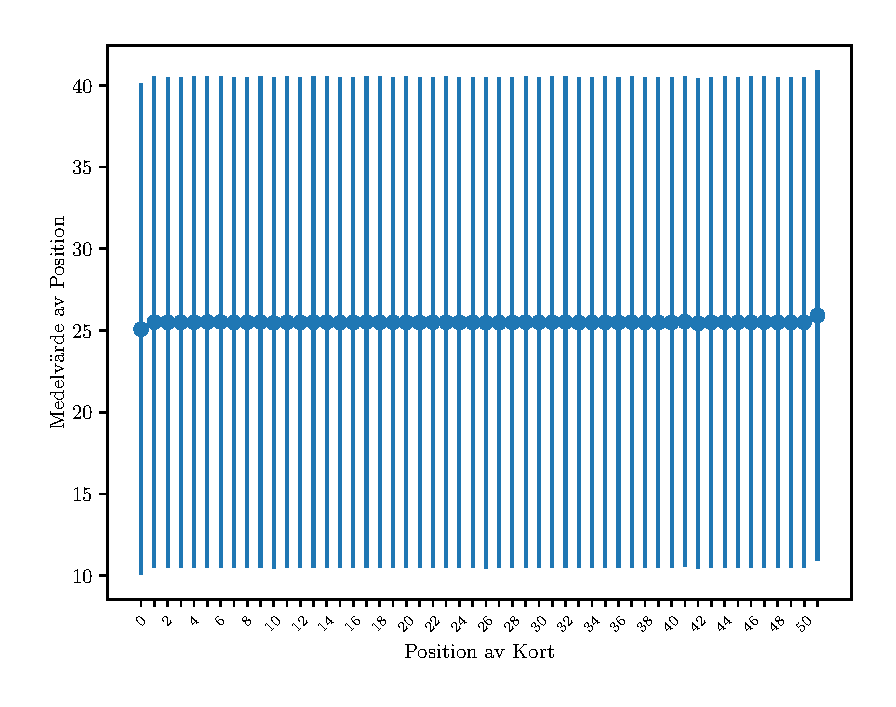
\includegraphics[width=0.8\textwidth, trim={0.8cm 0.8cm
	0.75cm 0.75cm}, clip]{soc_pile_shuffle-3} 
	\captionsetup{width=0.5\textwidth}
	\caption{Resultatet från \gls{stdmean} testet för \gls{soc} Pile
	Shuffle med \textbf{3} iterationer.}
	\label{fig:soc-3}
\end{figure}

\begin{figure}[H]
	\centering
	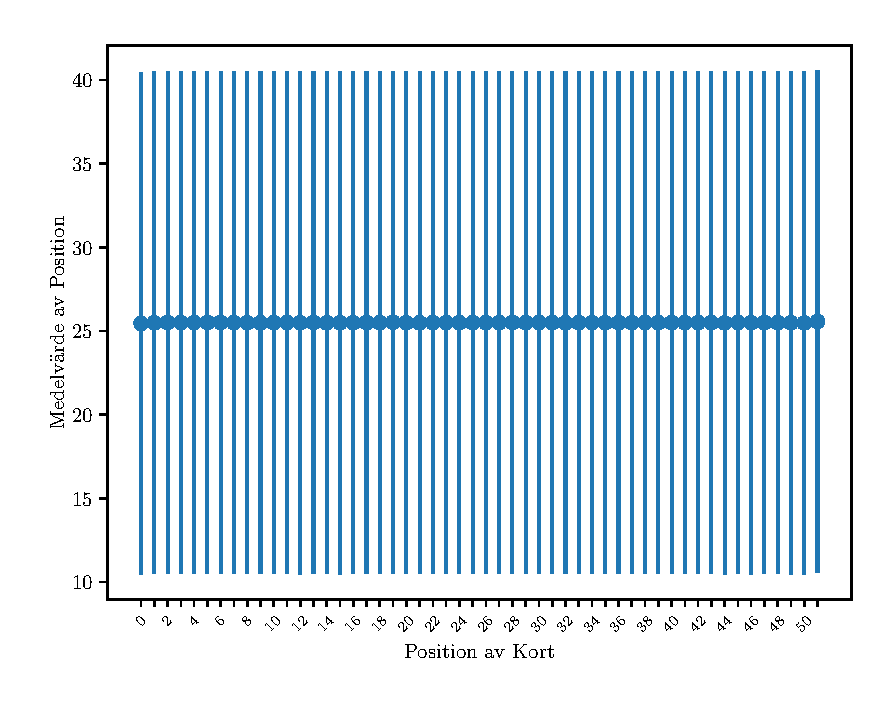
\includegraphics[width=0.8\textwidth, trim={0.8cm 0.8cm
	0.75cm 0.75cm}, clip]{soc_pile_shuffle-4} 
	\captionsetup{width=0.5\textwidth}
	\caption{Resultatet från \gls{stdmean} testet för \gls{soc} Pile
	Shuffle med \textbf{4} iterationer.}
	\label{fig:soc-4}
\end{figure}

\begin{figure}[H]
	\centering
	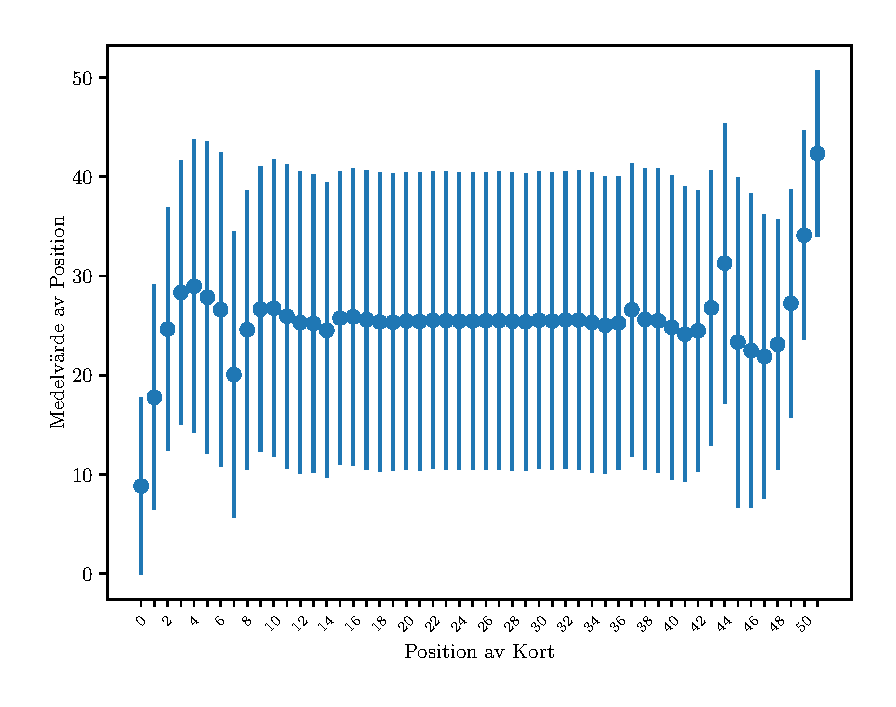
\includegraphics[width=0.8\textwidth, trim={0.8cm 0.8cm
	0.75cm 0.75cm}, clip]{ten_pile_shuffle-1} 
	\captionsetup{width=0.5\textwidth}
	\caption{Resultatet från \gls{stdmean} testet för Ten Pile
	Shuffle med \textbf{1} iteration.}
	\label{fig:ten-1}
\end{figure}

\begin{figure}[H]
	\centering
	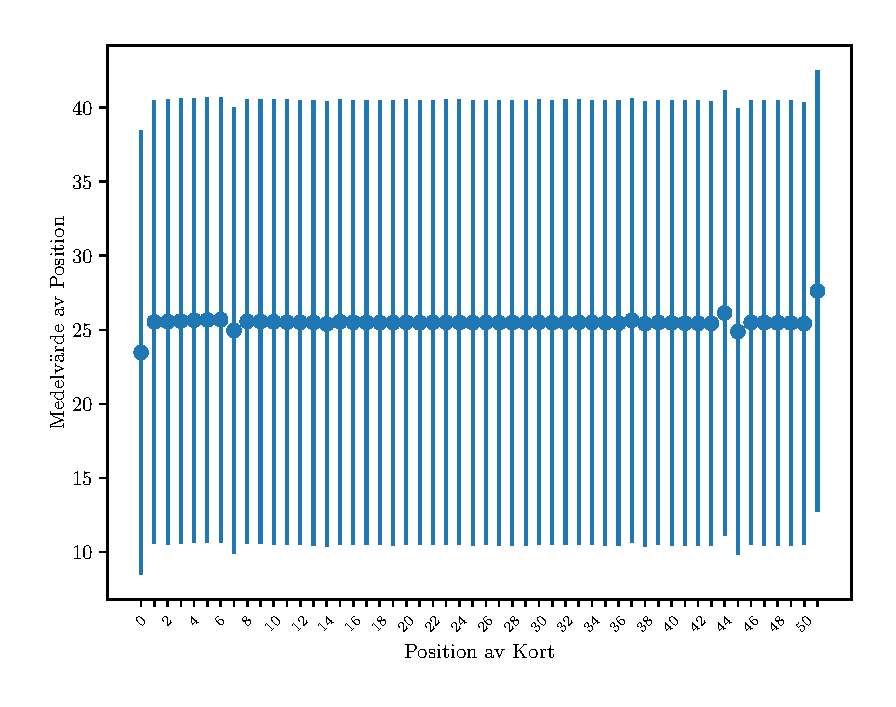
\includegraphics[width=0.8\textwidth, trim={0.8cm 0.8cm
	0.75cm 0.75cm}, clip]{ten_pile_shuffle-2} 
	\captionsetup{width=0.5\textwidth}
	\caption{Resultatet från \gls{stdmean} testet för Ten Pile
	Shuffle med \textbf{2} iterationer.}
	\label{fig:ten-2}
\end{figure}

\begin{figure}[H]
	\centering
	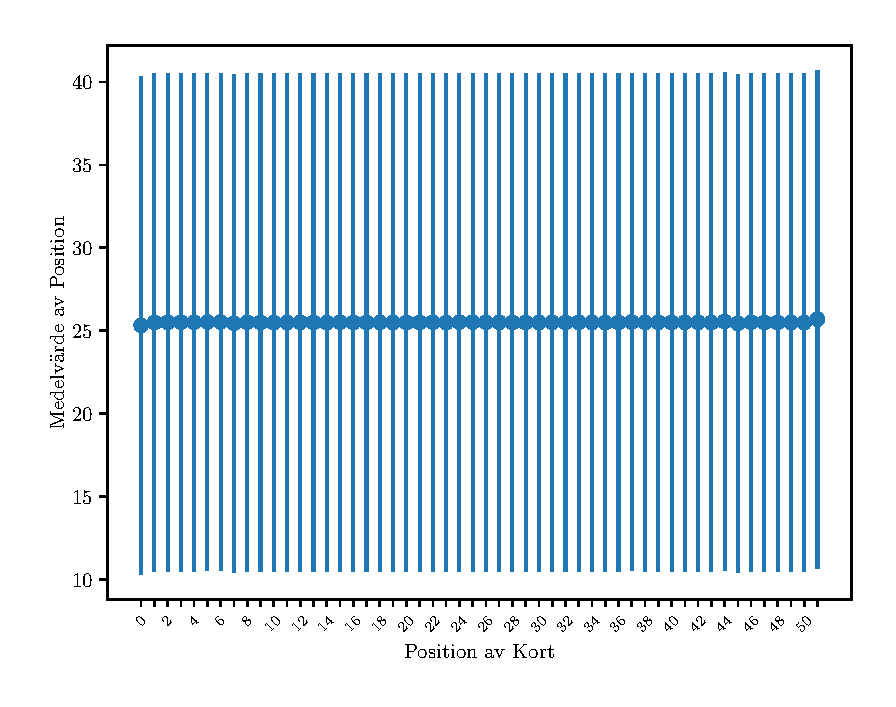
\includegraphics[width=0.8\textwidth, trim={0.8cm 0.8cm
	0.75cm 0.75cm}, clip]{ten_pile_shuffle-3} 
	\captionsetup{width=0.5\textwidth}
	\caption{Resultatet från \gls{stdmean} testet för Ten Pile
	Shuffle med \textbf{3} iterationer.}
	\label{fig:ten-3}
\end{figure}

\begin{figure}[H]
	\centering
	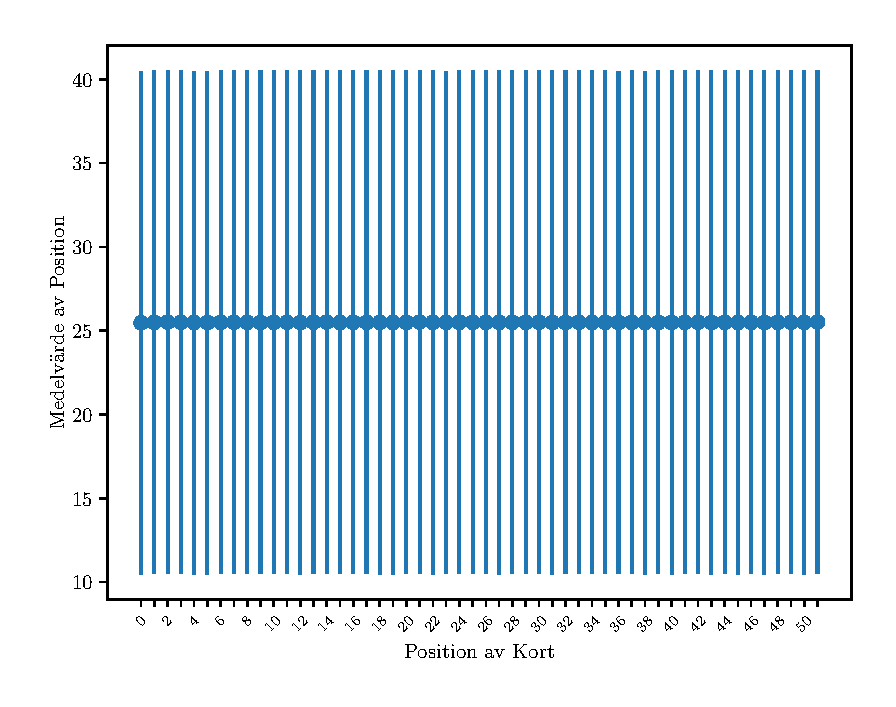
\includegraphics[width=0.8\textwidth, trim={0.8cm 0.8cm
	0.75cm 0.75cm}, clip]{ten_pile_shuffle-4} 
	\captionsetup{width=0.5\textwidth}
	\caption{Resultatet från \gls{stdmean} testet för Ten Pile
	Shuffle med \textbf{4} iterationer.}
	\label{fig:ten-4}
\end{figure}

\begin{figure}[H]
	\centering
	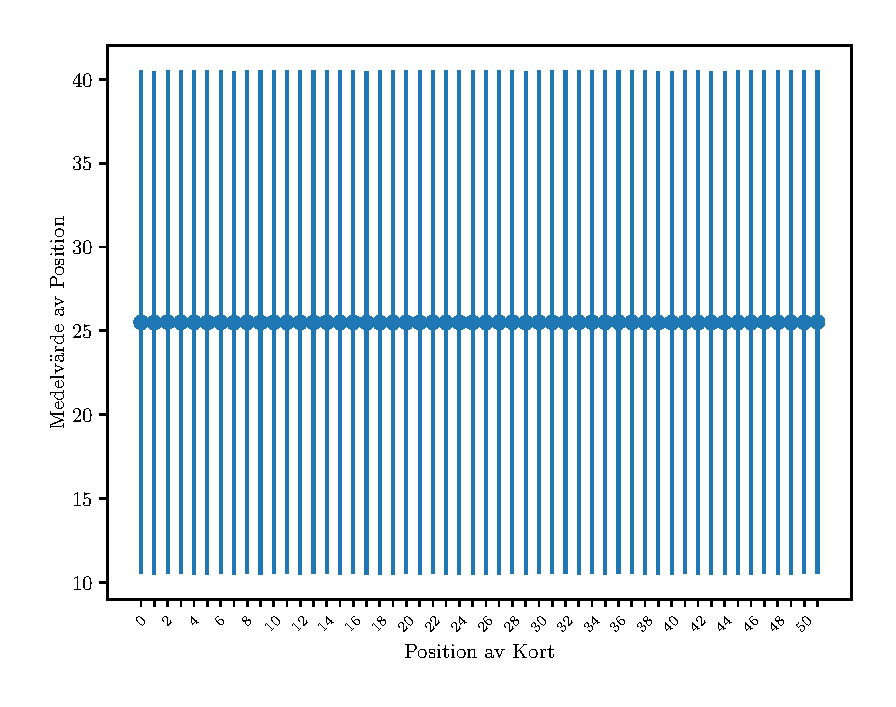
\includegraphics[width=0.8\textwidth, trim={0.8cm 0.8cm
	0.75cm 0.75cm}, clip]{wheel_spiny-1} 
	\captionsetup{width=0.5\textwidth}
	\caption{Resultatet från \gls{stdmean} testet för Wheel Fisher-Yates shuffle med \textbf{1} iteration.}
	\label{fig:wheel-1}
\end{figure}


\section{Diskussion}
Diskussion om resultaten av simulationerna är uppdelat i flera subsektioner i
syfte att göra det enklare att följa tankeproccesen lättare att följa. Den
första subsektionen handlar om hur den mest passade blandingsmetoden togs fram,
den här sektionen är updelad i två delar. Den preliminära gallringen är där dem
blandingsmetoder som är själklart ompassande gallras bort från undersökingen. I
jämförelsen av blandingesmetoderna kommer vi närmare undersöka dem metoder som
återstår efter gallringen för att komma fram till vilken av dem som passar bäst
inpå dem krav som ställdes i syftet \ref{sec:purpose}. Felkällor och källkritik
nämns efter att den mest passande blandningsmetoden tagit fram för att att
diskutera deras påverkan på dem tidgare slutsaterna i diskussionen. I slutsatsen
binds presenteras den blandningsmetod som undersökingen kom from till vad det
innebär och vilka förbättringar som skulle kunna göras i potentiell framtida
forskning.

\subsection{Den mest passande blandningsmetoden}

\subsubsection{Preliminär gallring}
Dem algoritmer som gallras är dem som helt säkert inte kommer vara bättre en dem
andra i dem färdigheterna som blandningsmetoderna jämförs på. Alla
blandningsmetoder som var signifikanta enligt chi-två-testet kan gallras då dem
inte uppnår en av kraven för blandningsmetoder, dem blandar inte på ett helt
slumpmässigt sätt.

\subsubsection{Jämförelse av blandningsmetoderna}


\subsection{Felkällor och Källkritik}


\subsection{Slutsats}


%\nocite{*}


\printbibliography[heading=bibintoc, title={Bibliografi}]
% \newpage

\appendix
\section*{\appendixpagename} 
\addcontentsline{toc}{section}{\appendixpagename} 

\section{Källkod}
\label{app:github}
Länk till Github repository vart Rust och Python källkod till simulationen 
respektive statistikst anlys är samlad, samt källkod till latex med
vilken detta rapport hade skrivits
länk: https://github.com/Abishevs/gymarbete

\section{Kod för GSR Riffle Shuffle}
\label{app:gsr}
% \lstinputlisting[language=Rust, caption={Pile Shuffle skriven i
% Rust},label=selection-sort, label={lst:gsr},firstline=179, lastline=214]{../simulation_rust/src/main.rs}
% \lstinputlisting[language=Rust, firstline=179, lastline=214]{../simulation_rust/src/main.rs}

\section{Kod för Pile Shuffle}
\label{app:pile}
% \lstinputlisting[language=Rust, firstline=29, lastline=55]{../simulation_rust/src/main.rs}

\section{Kod för Wheel Fisher-Yates shuffle}
\label{app:wheel}
% \lstinputlisting[language=Rust, firstline=147, lastline=167]{../simulation_rust/src/main.rs}

% \section{Template att bifoga ett inline kod}
% \label{sec:source_code}
% \begin{lstlisting}[language=Python, caption=Python example]
% # Your source code here
% print("Hello, World!")
% \end{lstlisting}

% \section{Template att bigoga källkod ifrån git repo}
% \label{app:source_code2}
%\lstinputlisting[language=Rust, caption={algorithm 1 implemention},label=selection-sort, label={lst:algo_1},firstline=24, lastline=50]{../simulation_rust/src/main.rs}


\end{document}
